% Options for packages loaded elsewhere
\PassOptionsToPackage{unicode}{hyperref}
\PassOptionsToPackage{hyphens}{url}
%
\documentclass[
]{article}
\usepackage{amsmath,amssymb}
\usepackage{lmodern}
\usepackage{iftex}
\ifPDFTeX
  \usepackage[T1]{fontenc}
  \usepackage[utf8]{inputenc}
  \usepackage{textcomp} % provide euro and other symbols
\else % if luatex or xetex
  \usepackage{unicode-math}
  \defaultfontfeatures{Scale=MatchLowercase}
  \defaultfontfeatures[\rmfamily]{Ligatures=TeX,Scale=1}
\fi
% Use upquote if available, for straight quotes in verbatim environments
\IfFileExists{upquote.sty}{\usepackage{upquote}}{}
\IfFileExists{microtype.sty}{% use microtype if available
  \usepackage[]{microtype}
  \UseMicrotypeSet[protrusion]{basicmath} % disable protrusion for tt fonts
}{}
\makeatletter
\@ifundefined{KOMAClassName}{% if non-KOMA class
  \IfFileExists{parskip.sty}{%
    \usepackage{parskip}
  }{% else
    \setlength{\parindent}{0pt}
    \setlength{\parskip}{6pt plus 2pt minus 1pt}}
}{% if KOMA class
  \KOMAoptions{parskip=half}}
\makeatother
\usepackage{xcolor}
\usepackage[margin=1in]{geometry}
\usepackage{color}
\usepackage{fancyvrb}
\newcommand{\VerbBar}{|}
\newcommand{\VERB}{\Verb[commandchars=\\\{\}]}
\DefineVerbatimEnvironment{Highlighting}{Verbatim}{commandchars=\\\{\}}
% Add ',fontsize=\small' for more characters per line
\usepackage{framed}
\definecolor{shadecolor}{RGB}{248,248,248}
\newenvironment{Shaded}{\begin{snugshade}}{\end{snugshade}}
\newcommand{\AlertTok}[1]{\textcolor[rgb]{0.94,0.16,0.16}{#1}}
\newcommand{\AnnotationTok}[1]{\textcolor[rgb]{0.56,0.35,0.01}{\textbf{\textit{#1}}}}
\newcommand{\AttributeTok}[1]{\textcolor[rgb]{0.77,0.63,0.00}{#1}}
\newcommand{\BaseNTok}[1]{\textcolor[rgb]{0.00,0.00,0.81}{#1}}
\newcommand{\BuiltInTok}[1]{#1}
\newcommand{\CharTok}[1]{\textcolor[rgb]{0.31,0.60,0.02}{#1}}
\newcommand{\CommentTok}[1]{\textcolor[rgb]{0.56,0.35,0.01}{\textit{#1}}}
\newcommand{\CommentVarTok}[1]{\textcolor[rgb]{0.56,0.35,0.01}{\textbf{\textit{#1}}}}
\newcommand{\ConstantTok}[1]{\textcolor[rgb]{0.00,0.00,0.00}{#1}}
\newcommand{\ControlFlowTok}[1]{\textcolor[rgb]{0.13,0.29,0.53}{\textbf{#1}}}
\newcommand{\DataTypeTok}[1]{\textcolor[rgb]{0.13,0.29,0.53}{#1}}
\newcommand{\DecValTok}[1]{\textcolor[rgb]{0.00,0.00,0.81}{#1}}
\newcommand{\DocumentationTok}[1]{\textcolor[rgb]{0.56,0.35,0.01}{\textbf{\textit{#1}}}}
\newcommand{\ErrorTok}[1]{\textcolor[rgb]{0.64,0.00,0.00}{\textbf{#1}}}
\newcommand{\ExtensionTok}[1]{#1}
\newcommand{\FloatTok}[1]{\textcolor[rgb]{0.00,0.00,0.81}{#1}}
\newcommand{\FunctionTok}[1]{\textcolor[rgb]{0.00,0.00,0.00}{#1}}
\newcommand{\ImportTok}[1]{#1}
\newcommand{\InformationTok}[1]{\textcolor[rgb]{0.56,0.35,0.01}{\textbf{\textit{#1}}}}
\newcommand{\KeywordTok}[1]{\textcolor[rgb]{0.13,0.29,0.53}{\textbf{#1}}}
\newcommand{\NormalTok}[1]{#1}
\newcommand{\OperatorTok}[1]{\textcolor[rgb]{0.81,0.36,0.00}{\textbf{#1}}}
\newcommand{\OtherTok}[1]{\textcolor[rgb]{0.56,0.35,0.01}{#1}}
\newcommand{\PreprocessorTok}[1]{\textcolor[rgb]{0.56,0.35,0.01}{\textit{#1}}}
\newcommand{\RegionMarkerTok}[1]{#1}
\newcommand{\SpecialCharTok}[1]{\textcolor[rgb]{0.00,0.00,0.00}{#1}}
\newcommand{\SpecialStringTok}[1]{\textcolor[rgb]{0.31,0.60,0.02}{#1}}
\newcommand{\StringTok}[1]{\textcolor[rgb]{0.31,0.60,0.02}{#1}}
\newcommand{\VariableTok}[1]{\textcolor[rgb]{0.00,0.00,0.00}{#1}}
\newcommand{\VerbatimStringTok}[1]{\textcolor[rgb]{0.31,0.60,0.02}{#1}}
\newcommand{\WarningTok}[1]{\textcolor[rgb]{0.56,0.35,0.01}{\textbf{\textit{#1}}}}
\usepackage{graphicx}
\makeatletter
\def\maxwidth{\ifdim\Gin@nat@width>\linewidth\linewidth\else\Gin@nat@width\fi}
\def\maxheight{\ifdim\Gin@nat@height>\textheight\textheight\else\Gin@nat@height\fi}
\makeatother
% Scale images if necessary, so that they will not overflow the page
% margins by default, and it is still possible to overwrite the defaults
% using explicit options in \includegraphics[width, height, ...]{}
\setkeys{Gin}{width=\maxwidth,height=\maxheight,keepaspectratio}
% Set default figure placement to htbp
\makeatletter
\def\fps@figure{htbp}
\makeatother
\setlength{\emergencystretch}{3em} % prevent overfull lines
\providecommand{\tightlist}{%
  \setlength{\itemsep}{0pt}\setlength{\parskip}{0pt}}
\setcounter{secnumdepth}{-\maxdimen} % remove section numbering
\ifLuaTeX
  \usepackage{selnolig}  % disable illegal ligatures
\fi
\IfFileExists{bookmark.sty}{\usepackage{bookmark}}{\usepackage{hyperref}}
\IfFileExists{xurl.sty}{\usepackage{xurl}}{} % add URL line breaks if available
\urlstyle{same} % disable monospaced font for URLs
\hypersetup{
  pdftitle={HUDM6026 Homework\_09},
  pdfauthor={Chenguang Pan},
  hidelinks,
  pdfcreator={LaTeX via pandoc}}

\title{HUDM6026 Homework\_09}
\author{Chenguang Pan}
\date{Mar 31, 2023}

\begin{document}
\maketitle

\hypertarget{q1-chapter-3.9}{%
\subsection{Q1: Chapter 3.9}\label{q1-chapter-3.9}}

\emph{Chapter 3, problem 9.Chapter 4, problems 1, 6, 13} \emph{This
question involves the use of multiple linear regression on the Auto data
set.}

\hypertarget{aproduce-a-scatterplot-matrix-which-includes-all-of-the-variables-in-the-data-set.}{%
\subsubsection{\texorpdfstring{\emph{(a)Produce a scatterplot matrix
which includes all of the variables in the data
set.}}{(a)Produce a scatterplot matrix which includes all of the variables in the data set.}}\label{aproduce-a-scatterplot-matrix-which-includes-all-of-the-variables-in-the-data-set.}}

\textbf{MY SOLUTION:}

\begin{Shaded}
\begin{Highlighting}[]
\SpecialCharTok{\textgreater{}} \CommentTok{\# import the package and the data}
\ErrorTok{\textgreater{}} \FunctionTok{library}\NormalTok{(ISLR2)}
\SpecialCharTok{\textgreater{}} \FunctionTok{data}\NormalTok{(Auto)}
\SpecialCharTok{\textgreater{}} \FunctionTok{pairs}\NormalTok{(Auto,}\AttributeTok{cex=}\FloatTok{0.5}\NormalTok{,}
\SpecialCharTok{+}       \AttributeTok{main =} \StringTok{"Firgue 1. Scatterplot matrix of Auto dataset"}\NormalTok{)}
\end{Highlighting}
\end{Shaded}

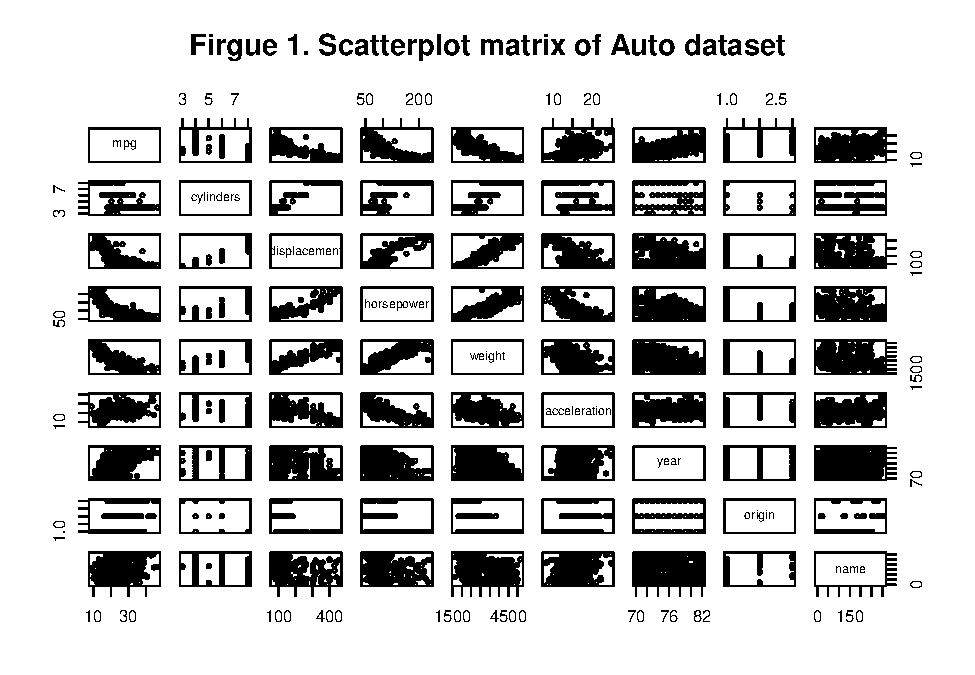
\includegraphics{Homework_09_new_Pan_files/figure-latex/unnamed-chunk-1-1.pdf}
Or, one can use the package \texttt{GGally} to make the scatterplot in a
more informative way. But before running this function, one should drop
the categorical variable \texttt{name} in case of warning. More details
can be found at \url{https://r-charts.com/correlation/ggpairs/} .

\begin{Shaded}
\begin{Highlighting}[]
\SpecialCharTok{\textgreater{}} \FunctionTok{library}\NormalTok{(GGally)}
\SpecialCharTok{\textgreater{}} \FunctionTok{colnames}\NormalTok{(Auto)}
\NormalTok{[}\DecValTok{1}\NormalTok{] }\StringTok{"mpg"}          \StringTok{"cylinders"}    \StringTok{"displacement"} \StringTok{"horsepower"}   \StringTok{"weight"}      
\NormalTok{[}\DecValTok{6}\NormalTok{] }\StringTok{"acceleration"} \StringTok{"year"}         \StringTok{"origin"}       \StringTok{"name"}        
\SpecialCharTok{\textgreater{}} \FunctionTok{ggpairs}\NormalTok{(Auto[,}\SpecialCharTok{{-}}\DecValTok{9}\NormalTok{], }\CommentTok{\# drop the name variable}
\SpecialCharTok{+}         \CommentTok{\# adjust the font size in the upper panel}
\SpecialCharTok{+}         \AttributeTok{upper =} \FunctionTok{list}\NormalTok{(}\AttributeTok{continuous=}\FunctionTok{wrap}\NormalTok{(}\StringTok{"cor"}\NormalTok{, }\AttributeTok{size =} \FloatTok{2.0}\NormalTok{)),}
\SpecialCharTok{+}         \CommentTok{\# add main title}
\SpecialCharTok{+}         \AttributeTok{title =}\StringTok{"Firgue 2. Scatterplot matrix of Auto dataset using ggpairs()"}\NormalTok{ )}
\end{Highlighting}
\end{Shaded}

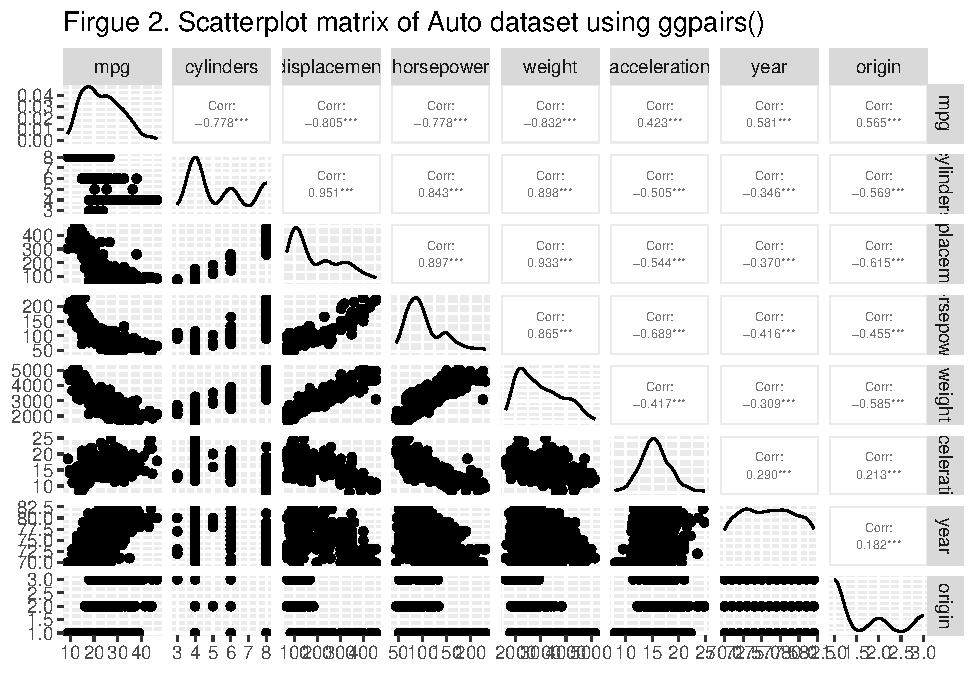
\includegraphics{Homework_09_new_Pan_files/figure-latex/unnamed-chunk-2-1.pdf}

\hypertarget{bcompute-the-matrix-of-correlations-between-the-variables-using-the-function-cor.-you-will-need-to-exclude-the-name-variable-which-is-qualitative}{%
\subsubsection{\texorpdfstring{\emph{(b)Compute the matrix of
correlations between the variables using the function cor(). You will
need to exclude the name variable, which is
qualitative}}{(b)Compute the matrix of correlations between the variables using the function cor(). You will need to exclude the name variable, which is qualitative}}\label{bcompute-the-matrix-of-correlations-between-the-variables-using-the-function-cor.-you-will-need-to-exclude-the-name-variable-which-is-qualitative}}

\textbf{MY SOLUTION:}\\
To make the corealtion matrix looking good, I abbreviated the variables'
names to save space.

\begin{Shaded}
\begin{Highlighting}[]
\SpecialCharTok{\textgreater{}} \CommentTok{\# save the matrix to cor\_mat}
\ErrorTok{\textgreater{}}\NormalTok{ cor\_mat }\OtherTok{\textless{}{-}} \FunctionTok{round}\NormalTok{(}\FunctionTok{cor}\NormalTok{(Auto[,}\SpecialCharTok{{-}}\DecValTok{9}\NormalTok{]),}\DecValTok{3}\NormalTok{)}
\SpecialCharTok{\textgreater{}} \CommentTok{\# abbreviate the variables\textquotesingle{} names}
\ErrorTok{\textgreater{}}\NormalTok{ names }\OtherTok{\textless{}{-}} \FunctionTok{abbreviate}\NormalTok{(}\FunctionTok{colnames}\NormalTok{(Auto[,}\SpecialCharTok{{-}}\DecValTok{9}\NormalTok{]),}\DecValTok{4}\NormalTok{)}
\SpecialCharTok{\textgreater{}} \FunctionTok{rownames}\NormalTok{(cor\_mat) }\OtherTok{\textless{}{-}}\NormalTok{ names}
\SpecialCharTok{\textgreater{}} \FunctionTok{colnames}\NormalTok{(cor\_mat) }\OtherTok{\textless{}{-}}\NormalTok{ names}
\SpecialCharTok{\textgreater{}}\NormalTok{ cor\_mat}
\NormalTok{        mpg   cyln   dspl   hrsp   wght   accl   year   orgn}
\NormalTok{mpg   }\FloatTok{1.000} \SpecialCharTok{{-}}\FloatTok{0.778} \SpecialCharTok{{-}}\FloatTok{0.805} \SpecialCharTok{{-}}\FloatTok{0.778} \SpecialCharTok{{-}}\FloatTok{0.832}  \FloatTok{0.423}  \FloatTok{0.581}  \FloatTok{0.565}
\NormalTok{cyln }\SpecialCharTok{{-}}\FloatTok{0.778}  \FloatTok{1.000}  \FloatTok{0.951}  \FloatTok{0.843}  \FloatTok{0.898} \SpecialCharTok{{-}}\FloatTok{0.505} \SpecialCharTok{{-}}\FloatTok{0.346} \SpecialCharTok{{-}}\FloatTok{0.569}
\NormalTok{dspl }\SpecialCharTok{{-}}\FloatTok{0.805}  \FloatTok{0.951}  \FloatTok{1.000}  \FloatTok{0.897}  \FloatTok{0.933} \SpecialCharTok{{-}}\FloatTok{0.544} \SpecialCharTok{{-}}\FloatTok{0.370} \SpecialCharTok{{-}}\FloatTok{0.615}
\NormalTok{hrsp }\SpecialCharTok{{-}}\FloatTok{0.778}  \FloatTok{0.843}  \FloatTok{0.897}  \FloatTok{1.000}  \FloatTok{0.865} \SpecialCharTok{{-}}\FloatTok{0.689} \SpecialCharTok{{-}}\FloatTok{0.416} \SpecialCharTok{{-}}\FloatTok{0.455}
\NormalTok{wght }\SpecialCharTok{{-}}\FloatTok{0.832}  \FloatTok{0.898}  \FloatTok{0.933}  \FloatTok{0.865}  \FloatTok{1.000} \SpecialCharTok{{-}}\FloatTok{0.417} \SpecialCharTok{{-}}\FloatTok{0.309} \SpecialCharTok{{-}}\FloatTok{0.585}
\NormalTok{accl  }\FloatTok{0.423} \SpecialCharTok{{-}}\FloatTok{0.505} \SpecialCharTok{{-}}\FloatTok{0.544} \SpecialCharTok{{-}}\FloatTok{0.689} \SpecialCharTok{{-}}\FloatTok{0.417}  \FloatTok{1.000}  \FloatTok{0.290}  \FloatTok{0.213}
\NormalTok{year  }\FloatTok{0.581} \SpecialCharTok{{-}}\FloatTok{0.346} \SpecialCharTok{{-}}\FloatTok{0.370} \SpecialCharTok{{-}}\FloatTok{0.416} \SpecialCharTok{{-}}\FloatTok{0.309}  \FloatTok{0.290}  \FloatTok{1.000}  \FloatTok{0.182}
\NormalTok{orgn  }\FloatTok{0.565} \SpecialCharTok{{-}}\FloatTok{0.569} \SpecialCharTok{{-}}\FloatTok{0.615} \SpecialCharTok{{-}}\FloatTok{0.455} \SpecialCharTok{{-}}\FloatTok{0.585}  \FloatTok{0.213}  \FloatTok{0.182}  \FloatTok{1.000}
\end{Highlighting}
\end{Shaded}

\hypertarget{c-use-the-lm-function-to-perform-a-multiple-linear-regression-with-mpg-as-the-response-and-all-other-variables-except-name-as-the-predictors.-use-the-summary-function-to-print-the-results.-comment-on-the-output.-for-instance}{%
\subsubsection{\texorpdfstring{\emph{(c) Use the lm() function to
perform a multiple linear regression with mpg as the response and all
other variables except name as the predictors. Use the summary()
function to print the results. Comment on the output. For
instance:}}{(c) Use the lm() function to perform a multiple linear regression with mpg as the response and all other variables except name as the predictors. Use the summary() function to print the results. Comment on the output. For instance:}}\label{c-use-the-lm-function-to-perform-a-multiple-linear-regression-with-mpg-as-the-response-and-all-other-variables-except-name-as-the-predictors.-use-the-summary-function-to-print-the-results.-comment-on-the-output.-for-instance}}

\textbf{MY SOLUTION:}

\begin{Shaded}
\begin{Highlighting}[]
\SpecialCharTok{\textgreater{}} \CommentTok{\# run the multiple linear regression model}
\ErrorTok{\textgreater{}}\NormalTok{ model\_01 }\OtherTok{\textless{}{-}} \FunctionTok{lm}\NormalTok{(mpg }\SpecialCharTok{\textasciitilde{}}\NormalTok{. }\SpecialCharTok{{-}}\NormalTok{name, }\AttributeTok{data =}\NormalTok{ Auto )}
\SpecialCharTok{\textgreater{}} \FunctionTok{summary}\NormalTok{(model\_01)}

\NormalTok{Call}\SpecialCharTok{:}
\FunctionTok{lm}\NormalTok{(}\AttributeTok{formula =}\NormalTok{ mpg }\SpecialCharTok{\textasciitilde{}}\NormalTok{ . }\SpecialCharTok{{-}}\NormalTok{ name, }\AttributeTok{data =}\NormalTok{ Auto)}

\NormalTok{Residuals}\SpecialCharTok{:}
\NormalTok{    Min      1Q  Median      3Q     Max }
\SpecialCharTok{{-}}\FloatTok{9.5903} \SpecialCharTok{{-}}\FloatTok{2.1565} \SpecialCharTok{{-}}\FloatTok{0.1169}  \FloatTok{1.8690} \FloatTok{13.0604} 

\NormalTok{Coefficients}\SpecialCharTok{:}
\NormalTok{               Estimate Std. Error t value }\FunctionTok{Pr}\NormalTok{(}\SpecialCharTok{\textgreater{}}\ErrorTok{|}\NormalTok{t}\SpecialCharTok{|}\NormalTok{)    }
\NormalTok{(Intercept)  }\SpecialCharTok{{-}}\FloatTok{17.218435}   \FloatTok{4.644294}  \SpecialCharTok{{-}}\FloatTok{3.707}  \FloatTok{0.00024} \SpecialCharTok{**}\ErrorTok{*}
\NormalTok{cylinders     }\SpecialCharTok{{-}}\FloatTok{0.493376}   \FloatTok{0.323282}  \SpecialCharTok{{-}}\FloatTok{1.526}  \FloatTok{0.12780}    
\NormalTok{displacement   }\FloatTok{0.019896}   \FloatTok{0.007515}   \FloatTok{2.647}  \FloatTok{0.00844} \SpecialCharTok{**} 
\NormalTok{horsepower    }\SpecialCharTok{{-}}\FloatTok{0.016951}   \FloatTok{0.013787}  \SpecialCharTok{{-}}\FloatTok{1.230}  \FloatTok{0.21963}    
\NormalTok{weight        }\SpecialCharTok{{-}}\FloatTok{0.006474}   \FloatTok{0.000652}  \SpecialCharTok{{-}}\FloatTok{9.929}  \SpecialCharTok{\textless{}} \FloatTok{2e{-}16} \SpecialCharTok{**}\ErrorTok{*}
\NormalTok{acceleration   }\FloatTok{0.080576}   \FloatTok{0.098845}   \FloatTok{0.815}  \FloatTok{0.41548}    
\NormalTok{year           }\FloatTok{0.750773}   \FloatTok{0.050973}  \FloatTok{14.729}  \SpecialCharTok{\textless{}} \FloatTok{2e{-}16} \SpecialCharTok{**}\ErrorTok{*}
\NormalTok{origin         }\FloatTok{1.426141}   \FloatTok{0.278136}   \FloatTok{5.127} \FloatTok{4.67e{-}07} \SpecialCharTok{**}\ErrorTok{*}
\SpecialCharTok{{-}{-}{-}}
\NormalTok{Signif. codes}\SpecialCharTok{:}  \DecValTok{0} \StringTok{\textquotesingle{}***\textquotesingle{}} \FloatTok{0.001} \StringTok{\textquotesingle{}**\textquotesingle{}} \FloatTok{0.01} \StringTok{\textquotesingle{}*\textquotesingle{}} \FloatTok{0.05} \StringTok{\textquotesingle{}.\textquotesingle{}} \FloatTok{0.1} \StringTok{\textquotesingle{} \textquotesingle{}} \DecValTok{1}

\NormalTok{Residual standard error}\SpecialCharTok{:} \FloatTok{3.328}\NormalTok{ on }\DecValTok{384}\NormalTok{ degrees of freedom}
\NormalTok{Multiple R}\SpecialCharTok{{-}}\NormalTok{squared}\SpecialCharTok{:}  \FloatTok{0.8215}\NormalTok{,    Adjusted R}\SpecialCharTok{{-}}\NormalTok{squared}\SpecialCharTok{:}  \FloatTok{0.8182} 
\NormalTok{F}\SpecialCharTok{{-}}\NormalTok{statistic}\SpecialCharTok{:} \FloatTok{252.4}\NormalTok{ on }\DecValTok{7}\NormalTok{ and }\DecValTok{384}\NormalTok{ DF,  p}\SpecialCharTok{{-}}\NormalTok{value}\SpecialCharTok{:} \ErrorTok{\textless{}} \FloatTok{2.2e{-}16}
\end{Highlighting}
\end{Shaded}

The multiple linear regression analysis results show that the overall
model can explain 82.15\% variance of the outcome variable \texttt{mpg},
and the mode predict the outcome well, \(F(7,384)=252.4\), \(p < .001\).
The variable \texttt{displacement}, \texttt{weight}, \texttt{year}, and
\texttt{origin} have a statistically significant relationship with the
outcome. Specifically, one year increase (i.e., the ) in \texttt{year}
variable will be associated with .75 increase in the \texttt{mpg} after
controlling for all other variables, \(t = 14.729\), \(p <.001\).

\hypertarget{duse-the-plot-function-to-produce-diagnostic-plots-of-the-linear-regression-fit.-comment-on-any-problems-you-see-with-the-fit.-do-the-residual-plots-suggest-any-unusually-large-outliers-does-the-leverage-plot-identify-any-observations-with-unusually-high-leverage}{%
\subsubsection{\texorpdfstring{\emph{(d)Use the plot() function to
produce diagnostic plots of the linear regression fit. Comment on any
problems you see with the fit. Do the residual plots suggest any
unusually large outliers? Does the leverage plot identify any
observations with unusually high
leverage?}}{(d)Use the plot() function to produce diagnostic plots of the linear regression fit. Comment on any problems you see with the fit. Do the residual plots suggest any unusually large outliers? Does the leverage plot identify any observations with unusually high leverage?}}\label{duse-the-plot-function-to-produce-diagnostic-plots-of-the-linear-regression-fit.-comment-on-any-problems-you-see-with-the-fit.-do-the-residual-plots-suggest-any-unusually-large-outliers-does-the-leverage-plot-identify-any-observations-with-unusually-high-leverage}}

\textbf{MY SOLUTION:}\\
Reference for this part
\url{https://www.andrew.cmu.edu/user/achoulde/94842/homework/regression_diagnostics.html}.\\
\url{http://www.h4labs.com/ml/islr/chapter03/03_09_melling.html}

\begin{Shaded}
\begin{Highlighting}[]
\SpecialCharTok{\textgreater{}} \FunctionTok{par}\NormalTok{(}\AttributeTok{mfrow=}\FunctionTok{c}\NormalTok{(}\DecValTok{2}\NormalTok{,}\DecValTok{2}\NormalTok{))}
\SpecialCharTok{\textgreater{}} \FunctionTok{plot}\NormalTok{(model\_01)}
\end{Highlighting}
\end{Shaded}

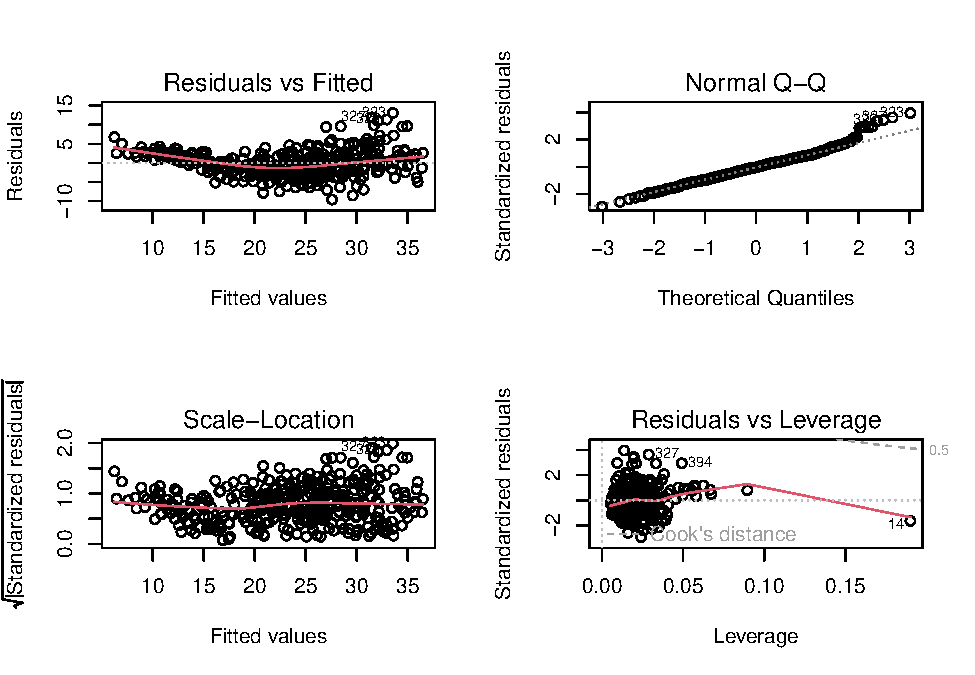
\includegraphics{Homework_09_new_Pan_files/figure-latex/unnamed-chunk-5-1.pdf}
The \emph{Residuals vs.~Fitted plot} shows that the average value of the
residuals at each value of fitted value (i.e., the red line) has a
U-shape pattern, which might indicate that the data is not linear. In
addition, the residuals presents non-equally distribution across the
entire range of fitted values. It is a sign of non-constant variance.

The \emph{normal Q-Q plot} shows that the residuals have a good normal
distribution despite some data points at the tails.

The \emph{scale-location plot} supports the findings from the
\emph{Residuals vs.~Fitted plot} that there is non-equal variance. Also,
it presents that there is no outlier since all values are within the
range of {[}-2,2{]}.

From the last plot, all data are well inside the Cook's distance lines
(red-dotted line). Therefore, there is no influential case (high
leverage data) in this dataset.

In conclusion, the diagnostic plots indicate the non-equal variance, no
outliers, and not high leverage data.

\hypertarget{euse-the-and-symbols-to-fit-linear-regression-models-with-interaction-effects.-do-any-interactions-appear-to-be-statistically-significant}{%
\subsubsection{\texorpdfstring{\emph{(e)Use the and : symbols to fit
linear regression models with interaction effects. Do any interactions
appear to be statistically
significant?}}{(e)Use the and : symbols to fit linear regression models with interaction effects. Do any interactions appear to be statistically significant?}}\label{euse-the-and-symbols-to-fit-linear-regression-models-with-interaction-effects.-do-any-interactions-appear-to-be-statistically-significant}}

\textbf{MY SOLUTION:}

Tips: What is the difference between the symbol \texttt{*} and
\texttt{:} in \texttt{lm()}?\\
The \texttt{*} symbol specifies that we want to include both the main
effect and the interaction term.
\texttt{lm(y\ \textasciitilde{}\ x\ *\ z)} equals
\texttt{lm(y\ \textasciitilde{}\ x\ +\ z\ +\ x:z)}.\\
The \texttt{:} symbol specifies that we want to include only the
interaction term. \texttt{lm(y\ \textasciitilde{}\ x\ :\ z)} equals
\texttt{lm(y\ \textasciitilde{}\ x*z\ -\ x\ -\ z)}.

\begin{Shaded}
\begin{Highlighting}[]
\SpecialCharTok{\textgreater{}} \FunctionTok{colnames}\NormalTok{(Auto)}
\NormalTok{[}\DecValTok{1}\NormalTok{] }\StringTok{"mpg"}          \StringTok{"cylinders"}    \StringTok{"displacement"} \StringTok{"horsepower"}   \StringTok{"weight"}      
\NormalTok{[}\DecValTok{6}\NormalTok{] }\StringTok{"acceleration"} \StringTok{"year"}         \StringTok{"origin"}       \StringTok{"name"}        
\SpecialCharTok{\textgreater{}}\NormalTok{ model\_02 }\OtherTok{\textless{}{-}} \FunctionTok{lm}\NormalTok{(mpg }\SpecialCharTok{\textasciitilde{}}\NormalTok{.}\SpecialCharTok{{-}}\NormalTok{name }\SpecialCharTok{+}\NormalTok{ horsepower}\SpecialCharTok{:}\NormalTok{weight, }\AttributeTok{data =}\NormalTok{ Auto)}
\SpecialCharTok{\textgreater{}}\NormalTok{ model\_03 }\OtherTok{\textless{}{-}} \FunctionTok{lm}\NormalTok{(mpg }\SpecialCharTok{\textasciitilde{}}\NormalTok{.}\SpecialCharTok{{-}}\NormalTok{name }\SpecialCharTok{+}\NormalTok{ horsepower}\SpecialCharTok{:}\NormalTok{origin, }\AttributeTok{data =}\NormalTok{ Auto)}
\SpecialCharTok{\textgreater{}} \FunctionTok{summary}\NormalTok{(model\_02)}

\NormalTok{Call}\SpecialCharTok{:}
\FunctionTok{lm}\NormalTok{(}\AttributeTok{formula =}\NormalTok{ mpg }\SpecialCharTok{\textasciitilde{}}\NormalTok{ . }\SpecialCharTok{{-}}\NormalTok{ name }\SpecialCharTok{+}\NormalTok{ horsepower}\SpecialCharTok{:}\NormalTok{weight, }\AttributeTok{data =}\NormalTok{ Auto)}

\NormalTok{Residuals}\SpecialCharTok{:}
\NormalTok{   Min     1Q Median     3Q    Max }
\SpecialCharTok{{-}}\FloatTok{8.589} \SpecialCharTok{{-}}\FloatTok{1.617} \SpecialCharTok{{-}}\FloatTok{0.184}  \FloatTok{1.541} \FloatTok{12.001} 

\NormalTok{Coefficients}\SpecialCharTok{:}
\NormalTok{                    Estimate Std. Error t value }\FunctionTok{Pr}\NormalTok{(}\SpecialCharTok{\textgreater{}}\ErrorTok{|}\NormalTok{t}\SpecialCharTok{|}\NormalTok{)    }
\NormalTok{(Intercept)        }\FloatTok{2.876e+00}  \FloatTok{4.511e+00}   \FloatTok{0.638} \FloatTok{0.524147}    
\NormalTok{cylinders         }\SpecialCharTok{{-}}\FloatTok{2.955e{-}02}  \FloatTok{2.881e{-}01}  \SpecialCharTok{{-}}\FloatTok{0.103} \FloatTok{0.918363}    
\NormalTok{displacement       }\FloatTok{5.950e{-}03}  \FloatTok{6.750e{-}03}   \FloatTok{0.881} \FloatTok{0.378610}    
\NormalTok{horsepower        }\SpecialCharTok{{-}}\FloatTok{2.313e{-}01}  \FloatTok{2.363e{-}02}  \SpecialCharTok{{-}}\FloatTok{9.791}  \SpecialCharTok{\textless{}} \FloatTok{2e{-}16} \SpecialCharTok{**}\ErrorTok{*}
\NormalTok{weight            }\SpecialCharTok{{-}}\FloatTok{1.121e{-}02}  \FloatTok{7.285e{-}04} \SpecialCharTok{{-}}\FloatTok{15.393}  \SpecialCharTok{\textless{}} \FloatTok{2e{-}16} \SpecialCharTok{**}\ErrorTok{*}
\NormalTok{acceleration      }\SpecialCharTok{{-}}\FloatTok{9.019e{-}02}  \FloatTok{8.855e{-}02}  \SpecialCharTok{{-}}\FloatTok{1.019} \FloatTok{0.309081}    
\NormalTok{year               }\FloatTok{7.695e{-}01}  \FloatTok{4.494e{-}02}  \FloatTok{17.124}  \SpecialCharTok{\textless{}} \FloatTok{2e{-}16} \SpecialCharTok{**}\ErrorTok{*}
\NormalTok{origin             }\FloatTok{8.344e{-}01}  \FloatTok{2.513e{-}01}   \FloatTok{3.320} \FloatTok{0.000986} \SpecialCharTok{**}\ErrorTok{*}
\NormalTok{horsepower}\SpecialCharTok{:}\NormalTok{weight  }\FloatTok{5.529e{-}05}  \FloatTok{5.227e{-}06}  \FloatTok{10.577}  \SpecialCharTok{\textless{}} \FloatTok{2e{-}16} \SpecialCharTok{**}\ErrorTok{*}
\SpecialCharTok{{-}{-}{-}}
\NormalTok{Signif. codes}\SpecialCharTok{:}  \DecValTok{0} \StringTok{\textquotesingle{}***\textquotesingle{}} \FloatTok{0.001} \StringTok{\textquotesingle{}**\textquotesingle{}} \FloatTok{0.01} \StringTok{\textquotesingle{}*\textquotesingle{}} \FloatTok{0.05} \StringTok{\textquotesingle{}.\textquotesingle{}} \FloatTok{0.1} \StringTok{\textquotesingle{} \textquotesingle{}} \DecValTok{1}

\NormalTok{Residual standard error}\SpecialCharTok{:} \FloatTok{2.931}\NormalTok{ on }\DecValTok{383}\NormalTok{ degrees of freedom}
\NormalTok{Multiple R}\SpecialCharTok{{-}}\NormalTok{squared}\SpecialCharTok{:}  \FloatTok{0.8618}\NormalTok{,    Adjusted R}\SpecialCharTok{{-}}\NormalTok{squared}\SpecialCharTok{:}  \FloatTok{0.859} 
\NormalTok{F}\SpecialCharTok{{-}}\NormalTok{statistic}\SpecialCharTok{:} \FloatTok{298.6}\NormalTok{ on }\DecValTok{8}\NormalTok{ and }\DecValTok{383}\NormalTok{ DF,  p}\SpecialCharTok{{-}}\NormalTok{value}\SpecialCharTok{:} \ErrorTok{\textless{}} \FloatTok{2.2e{-}16}
\SpecialCharTok{\textgreater{}} \FunctionTok{summary}\NormalTok{(model\_03)}

\NormalTok{Call}\SpecialCharTok{:}
\FunctionTok{lm}\NormalTok{(}\AttributeTok{formula =}\NormalTok{ mpg }\SpecialCharTok{\textasciitilde{}}\NormalTok{ . }\SpecialCharTok{{-}}\NormalTok{ name }\SpecialCharTok{+}\NormalTok{ horsepower}\SpecialCharTok{:}\NormalTok{origin, }\AttributeTok{data =}\NormalTok{ Auto)}

\NormalTok{Residuals}\SpecialCharTok{:}
\NormalTok{   Min     1Q Median     3Q    Max }
\SpecialCharTok{{-}}\FloatTok{9.277} \SpecialCharTok{{-}}\FloatTok{1.875} \SpecialCharTok{{-}}\FloatTok{0.225}  \FloatTok{1.570} \FloatTok{12.080} 

\NormalTok{Coefficients}\SpecialCharTok{:}
\NormalTok{                    Estimate Std. Error t value }\FunctionTok{Pr}\NormalTok{(}\SpecialCharTok{\textgreater{}}\ErrorTok{|}\NormalTok{t}\SpecialCharTok{|}\NormalTok{)    }
\NormalTok{(Intercept)       }\SpecialCharTok{{-}}\FloatTok{2.196e+01}  \FloatTok{4.396e+00}  \SpecialCharTok{{-}}\FloatTok{4.996} \FloatTok{8.94e{-}07} \SpecialCharTok{**}\ErrorTok{*}
\NormalTok{cylinders         }\SpecialCharTok{{-}}\FloatTok{5.275e{-}01}  \FloatTok{3.028e{-}01}  \SpecialCharTok{{-}}\FloatTok{1.742}   \FloatTok{0.0823}\NormalTok{ .  }
\NormalTok{displacement      }\SpecialCharTok{{-}}\FloatTok{1.486e{-}03}  \FloatTok{7.607e{-}03}  \SpecialCharTok{{-}}\FloatTok{0.195}   \FloatTok{0.8452}    
\NormalTok{horsepower         }\FloatTok{8.173e{-}02}  \FloatTok{1.856e{-}02}   \FloatTok{4.404} \FloatTok{1.38e{-}05} \SpecialCharTok{**}\ErrorTok{*}
\NormalTok{weight            }\SpecialCharTok{{-}}\FloatTok{4.710e{-}03}  \FloatTok{6.555e{-}04}  \SpecialCharTok{{-}}\FloatTok{7.186} \FloatTok{3.52e{-}12} \SpecialCharTok{**}\ErrorTok{*}
\NormalTok{acceleration      }\SpecialCharTok{{-}}\FloatTok{1.124e{-}01}  \FloatTok{9.617e{-}02}  \SpecialCharTok{{-}}\FloatTok{1.168}   \FloatTok{0.2434}    
\NormalTok{year               }\FloatTok{7.327e{-}01}  \FloatTok{4.780e{-}02}  \FloatTok{15.328}  \SpecialCharTok{\textless{}} \FloatTok{2e{-}16} \SpecialCharTok{**}\ErrorTok{*}
\NormalTok{origin             }\FloatTok{7.695e+00}  \FloatTok{8.858e{-}01}   \FloatTok{8.687}  \SpecialCharTok{\textless{}} \FloatTok{2e{-}16} \SpecialCharTok{**}\ErrorTok{*}
\NormalTok{horsepower}\SpecialCharTok{:}\NormalTok{origin }\SpecialCharTok{{-}}\FloatTok{7.955e{-}02}  \FloatTok{1.074e{-}02}  \SpecialCharTok{{-}}\FloatTok{7.405} \FloatTok{8.44e{-}13} \SpecialCharTok{**}\ErrorTok{*}
\SpecialCharTok{{-}{-}{-}}
\NormalTok{Signif. codes}\SpecialCharTok{:}  \DecValTok{0} \StringTok{\textquotesingle{}***\textquotesingle{}} \FloatTok{0.001} \StringTok{\textquotesingle{}**\textquotesingle{}} \FloatTok{0.01} \StringTok{\textquotesingle{}*\textquotesingle{}} \FloatTok{0.05} \StringTok{\textquotesingle{}.\textquotesingle{}} \FloatTok{0.1} \StringTok{\textquotesingle{} \textquotesingle{}} \DecValTok{1}

\NormalTok{Residual standard error}\SpecialCharTok{:} \FloatTok{3.116}\NormalTok{ on }\DecValTok{383}\NormalTok{ degrees of freedom}
\NormalTok{Multiple R}\SpecialCharTok{{-}}\NormalTok{squared}\SpecialCharTok{:}  \FloatTok{0.8438}\NormalTok{,    Adjusted R}\SpecialCharTok{{-}}\NormalTok{squared}\SpecialCharTok{:}  \FloatTok{0.8406} 
\NormalTok{F}\SpecialCharTok{{-}}\NormalTok{statistic}\SpecialCharTok{:} \FloatTok{258.7}\NormalTok{ on }\DecValTok{8}\NormalTok{ and }\DecValTok{383}\NormalTok{ DF,  p}\SpecialCharTok{{-}}\NormalTok{value}\SpecialCharTok{:} \ErrorTok{\textless{}} \FloatTok{2.2e{-}16}
\end{Highlighting}
\end{Shaded}

The two models presents the statistically significant interactions
between the \texttt{horsepower} and \texttt{weight}, also the
\texttt{horsepower} and \texttt{origin}.

\hypertarget{ftry-a-few-different-transformations-of-the-variables}{%
\subsubsection{\texorpdfstring{\emph{(f)Try a few different
transformations of the
variables}}{(f)Try a few different transformations of the variables}}\label{ftry-a-few-different-transformations-of-the-variables}}

\textbf{MY SOLUTION:}

\begin{Shaded}
\begin{Highlighting}[]
\SpecialCharTok{\textgreater{}}\NormalTok{ model\_04 }\OtherTok{\textless{}{-}} \FunctionTok{lm}\NormalTok{(mpg }\SpecialCharTok{\textasciitilde{}}\NormalTok{.}\SpecialCharTok{{-}}\NormalTok{name }\SpecialCharTok{+} \FunctionTok{I}\NormalTok{(horsepower}\SpecialCharTok{\^{}}\DecValTok{2}\NormalTok{)}\SpecialCharTok{+}\FunctionTok{I}\NormalTok{(horsepower}\SpecialCharTok{\^{}}\DecValTok{3}\NormalTok{),}\AttributeTok{data =}\NormalTok{ Auto)}
\SpecialCharTok{\textgreater{}} \FunctionTok{summary}\NormalTok{(model\_04)}

\NormalTok{Call}\SpecialCharTok{:}
\FunctionTok{lm}\NormalTok{(}\AttributeTok{formula =}\NormalTok{ mpg }\SpecialCharTok{\textasciitilde{}}\NormalTok{ . }\SpecialCharTok{{-}}\NormalTok{ name }\SpecialCharTok{+} \FunctionTok{I}\NormalTok{(horsepower}\SpecialCharTok{\^{}}\DecValTok{2}\NormalTok{) }\SpecialCharTok{+} \FunctionTok{I}\NormalTok{(horsepower}\SpecialCharTok{\^{}}\DecValTok{3}\NormalTok{), }
    \AttributeTok{data =}\NormalTok{ Auto)}

\NormalTok{Residuals}\SpecialCharTok{:}
\NormalTok{    Min      1Q  Median      3Q     Max }
\SpecialCharTok{{-}}\FloatTok{8.5280} \SpecialCharTok{{-}}\FloatTok{1.6612} \SpecialCharTok{{-}}\FloatTok{0.0408}  \FloatTok{1.4789} \FloatTok{11.9022} 

\NormalTok{Coefficients}\SpecialCharTok{:}
\NormalTok{                  Estimate Std. Error t value }\FunctionTok{Pr}\NormalTok{(}\SpecialCharTok{\textgreater{}}\ErrorTok{|}\NormalTok{t}\SpecialCharTok{|}\NormalTok{)    }
\NormalTok{(Intercept)      }\FloatTok{1.326e+01}  \FloatTok{5.486e+00}   \FloatTok{2.417} \FloatTok{0.016107} \SpecialCharTok{*}  
\NormalTok{cylinders       }\SpecialCharTok{{-}}\FloatTok{1.337e{-}01}  \FloatTok{3.242e{-}01}  \SpecialCharTok{{-}}\FloatTok{0.412} \FloatTok{0.680207}    
\NormalTok{displacement    }\SpecialCharTok{{-}}\FloatTok{3.516e{-}03}  \FloatTok{7.316e{-}03}  \SpecialCharTok{{-}}\FloatTok{0.481} \FloatTok{0.631083}    
\NormalTok{horsepower      }\SpecialCharTok{{-}}\FloatTok{6.284e{-}01}  \FloatTok{8.646e{-}02}  \SpecialCharTok{{-}}\FloatTok{7.268} \FloatTok{2.07e{-}12} \SpecialCharTok{**}\ErrorTok{*}
\NormalTok{weight          }\SpecialCharTok{{-}}\FloatTok{3.524e{-}03}  \FloatTok{6.697e{-}04}  \SpecialCharTok{{-}}\FloatTok{5.262} \FloatTok{2.39e{-}07} \SpecialCharTok{**}\ErrorTok{*}
\NormalTok{acceleration    }\SpecialCharTok{{-}}\FloatTok{2.994e{-}01}  \FloatTok{9.774e{-}02}  \SpecialCharTok{{-}}\FloatTok{3.063} \FloatTok{0.002343} \SpecialCharTok{**} 
\NormalTok{year             }\FloatTok{7.429e{-}01}  \FloatTok{4.521e{-}02}  \FloatTok{16.432}  \SpecialCharTok{\textless{}} \FloatTok{2e{-}16} \SpecialCharTok{**}\ErrorTok{*}
\NormalTok{origin           }\FloatTok{8.699e{-}01}  \FloatTok{2.528e{-}01}   \FloatTok{3.441} \FloatTok{0.000643} \SpecialCharTok{**}\ErrorTok{*}
\FunctionTok{I}\NormalTok{(horsepower}\SpecialCharTok{\^{}}\DecValTok{2}\NormalTok{)  }\FloatTok{3.744e{-}03}  \FloatTok{7.134e{-}04}   \FloatTok{5.249} \FloatTok{2.55e{-}07} \SpecialCharTok{**}\ErrorTok{*}
\FunctionTok{I}\NormalTok{(horsepower}\SpecialCharTok{\^{}}\DecValTok{3}\NormalTok{) }\SpecialCharTok{{-}}\FloatTok{7.103e{-}06}  \FloatTok{1.831e{-}06}  \SpecialCharTok{{-}}\FloatTok{3.881} \FloatTok{0.000123} \SpecialCharTok{**}\ErrorTok{*}
\SpecialCharTok{{-}{-}{-}}
\NormalTok{Signif. codes}\SpecialCharTok{:}  \DecValTok{0} \StringTok{\textquotesingle{}***\textquotesingle{}} \FloatTok{0.001} \StringTok{\textquotesingle{}**\textquotesingle{}} \FloatTok{0.01} \StringTok{\textquotesingle{}*\textquotesingle{}} \FloatTok{0.05} \StringTok{\textquotesingle{}.\textquotesingle{}} \FloatTok{0.1} \StringTok{\textquotesingle{} \textquotesingle{}} \DecValTok{1}

\NormalTok{Residual standard error}\SpecialCharTok{:} \FloatTok{2.947}\NormalTok{ on }\DecValTok{382}\NormalTok{ degrees of freedom}
\NormalTok{Multiple R}\SpecialCharTok{{-}}\NormalTok{squared}\SpecialCharTok{:}  \FloatTok{0.8607}\NormalTok{,    Adjusted R}\SpecialCharTok{{-}}\NormalTok{squared}\SpecialCharTok{:}  \FloatTok{0.8574} 
\NormalTok{F}\SpecialCharTok{{-}}\NormalTok{statistic}\SpecialCharTok{:} \FloatTok{262.3}\NormalTok{ on }\DecValTok{9}\NormalTok{ and }\DecValTok{382}\NormalTok{ DF,  p}\SpecialCharTok{{-}}\NormalTok{value}\SpecialCharTok{:} \ErrorTok{\textless{}} \FloatTok{2.2e{-}16}
\SpecialCharTok{\textgreater{}}\NormalTok{ model\_05 }\OtherTok{\textless{}{-}} \FunctionTok{lm}\NormalTok{(mpg }\SpecialCharTok{\textasciitilde{}}\NormalTok{.}\SpecialCharTok{{-}}\NormalTok{name }\SpecialCharTok{+} \FunctionTok{log}\NormalTok{(horsepower),}\AttributeTok{data =}\NormalTok{ Auto)}
\SpecialCharTok{\textgreater{}} \FunctionTok{summary}\NormalTok{(model\_05)}

\NormalTok{Call}\SpecialCharTok{:}
\FunctionTok{lm}\NormalTok{(}\AttributeTok{formula =}\NormalTok{ mpg }\SpecialCharTok{\textasciitilde{}}\NormalTok{ . }\SpecialCharTok{{-}}\NormalTok{ name }\SpecialCharTok{+} \FunctionTok{log}\NormalTok{(horsepower), }\AttributeTok{data =}\NormalTok{ Auto)}

\NormalTok{Residuals}\SpecialCharTok{:}
\NormalTok{    Min      1Q  Median      3Q     Max }
\SpecialCharTok{{-}}\FloatTok{8.5777} \SpecialCharTok{{-}}\FloatTok{1.6623} \SpecialCharTok{{-}}\FloatTok{0.1213}  \FloatTok{1.4913} \FloatTok{12.0230} 

\NormalTok{Coefficients}\SpecialCharTok{:}
\NormalTok{                  Estimate Std. Error t value }\FunctionTok{Pr}\NormalTok{(}\SpecialCharTok{\textgreater{}}\ErrorTok{|}\NormalTok{t}\SpecialCharTok{|}\NormalTok{)    }
\NormalTok{(Intercept)      }\FloatTok{8.674e+01}  \FloatTok{1.106e+01}   \FloatTok{7.839} \FloatTok{4.54e{-}14} \SpecialCharTok{**}\ErrorTok{*}
\NormalTok{cylinders       }\SpecialCharTok{{-}}\FloatTok{5.530e{-}02}  \FloatTok{2.907e{-}01}  \SpecialCharTok{{-}}\FloatTok{0.190} \FloatTok{0.849230}    
\NormalTok{displacement    }\SpecialCharTok{{-}}\FloatTok{4.607e{-}03}  \FloatTok{7.108e{-}03}  \SpecialCharTok{{-}}\FloatTok{0.648} \FloatTok{0.517291}    
\NormalTok{horsepower       }\FloatTok{1.764e{-}01}  \FloatTok{2.269e{-}02}   \FloatTok{7.775} \FloatTok{7.05e{-}14} \SpecialCharTok{**}\ErrorTok{*}
\NormalTok{weight          }\SpecialCharTok{{-}}\FloatTok{3.366e{-}03}  \FloatTok{6.561e{-}04}  \SpecialCharTok{{-}}\FloatTok{5.130} \FloatTok{4.62e{-}07} \SpecialCharTok{**}\ErrorTok{*}
\NormalTok{acceleration    }\SpecialCharTok{{-}}\FloatTok{3.277e{-}01}  \FloatTok{9.670e{-}02}  \SpecialCharTok{{-}}\FloatTok{3.388} \FloatTok{0.000776} \SpecialCharTok{**}\ErrorTok{*}
\NormalTok{year             }\FloatTok{7.421e{-}01}  \FloatTok{4.534e{-}02}  \FloatTok{16.368}  \SpecialCharTok{\textless{}} \FloatTok{2e{-}16} \SpecialCharTok{**}\ErrorTok{*}
\NormalTok{origin           }\FloatTok{8.976e{-}01}  \FloatTok{2.528e{-}01}   \FloatTok{3.551} \FloatTok{0.000432} \SpecialCharTok{**}\ErrorTok{*}
\FunctionTok{log}\NormalTok{(horsepower) }\SpecialCharTok{{-}}\FloatTok{2.685e+01}  \FloatTok{2.652e+00} \SpecialCharTok{{-}}\FloatTok{10.127}  \SpecialCharTok{\textless{}} \FloatTok{2e{-}16} \SpecialCharTok{**}\ErrorTok{*}
\SpecialCharTok{{-}{-}{-}}
\NormalTok{Signif. codes}\SpecialCharTok{:}  \DecValTok{0} \StringTok{\textquotesingle{}***\textquotesingle{}} \FloatTok{0.001} \StringTok{\textquotesingle{}**\textquotesingle{}} \FloatTok{0.01} \StringTok{\textquotesingle{}*\textquotesingle{}} \FloatTok{0.05} \StringTok{\textquotesingle{}.\textquotesingle{}} \FloatTok{0.1} \StringTok{\textquotesingle{} \textquotesingle{}} \DecValTok{1}

\NormalTok{Residual standard error}\SpecialCharTok{:} \FloatTok{2.959}\NormalTok{ on }\DecValTok{383}\NormalTok{ degrees of freedom}
\NormalTok{Multiple R}\SpecialCharTok{{-}}\NormalTok{squared}\SpecialCharTok{:}  \FloatTok{0.8592}\NormalTok{,    Adjusted R}\SpecialCharTok{{-}}\NormalTok{squared}\SpecialCharTok{:}  \FloatTok{0.8562} 
\NormalTok{F}\SpecialCharTok{{-}}\NormalTok{statistic}\SpecialCharTok{:} \FloatTok{292.1}\NormalTok{ on }\DecValTok{8}\NormalTok{ and }\DecValTok{383}\NormalTok{ DF,  p}\SpecialCharTok{{-}}\NormalTok{value}\SpecialCharTok{:} \ErrorTok{\textless{}} \FloatTok{2.2e{-}16}
\end{Highlighting}
\end{Shaded}

Here, I tried to add the different transformations of
\texttt{horsepower} variable. All models can explain the outcome well,
as all p-values are less than .001. Besides, referring to the
\(adjusted R^2\), the \texttt{model\_04} with the quadratic and cubic
form with \texttt{horsepower} has the best performance,
\(adjusted R^2=.8574\).

\hypertarget{q2-chapter-4.1}{%
\subsection{Q2: Chapter 4.1}\label{q2-chapter-4.1}}

\emph{Using a little bit of algebra, prove that (4.2) is equivalent to
(4.3). In other words, the logistic function representation and logit
represen- tation for the logistic regression model are equivalent}

\textbf{MY SOLUTION}\\
For typing convenience, let \(A= e^{\beta_0+\beta_1X}\). Therefore, the
formular (4.2) can be written as \(p(X) = \frac{A}{1+A}\). This
form-changing is similar to get the inverse function for \(p(X)\). That
is, we suppose that \(A\) is the function of \(p(x)\). Thus, we can have
\[p(X) + p(X)A = A,\]\[A[1-p(X)]=p(X).\] Then we have
\[A=\frac{p(X)}{1-P(X)}.\] After changing the A into the original form,
finally we have \[e^{\beta_0+\beta_1X} = \frac{p(X)}{1-p(X)}.\]

\hypertarget{q3-chapter-4.6}{%
\subsection{Q3: Chapter 4.6}\label{q3-chapter-4.6}}

\emph{Suppose we collect data for a group of students in a statistics
class with variables X1 = hours studied, X2 = undergrad GPA, and Y =
receive an A. We fit a logistic regression and produce estimated
coefficient}

\hypertarget{aestimate-the-probability-that-a-student-who-studies-for-40-h-and-has-an-undergrad-gpa-of-3.5-gets-an-a-in-the-class.}{%
\subsubsection{\texorpdfstring{\textbf{(a)Estimate the probability that
a student who studies for 40 h and has an undergrad GPA of 3.5 gets an A
in the
class.}}{(a)Estimate the probability that a student who studies for 40 h and has an undergrad GPA of 3.5 gets an A in the class.}}\label{aestimate-the-probability-that-a-student-who-studies-for-40-h-and-has-an-undergrad-gpa-of-3.5-gets-an-a-in-the-class.}}

\textbf{MY SOLUTION}

\begin{Shaded}
\begin{Highlighting}[]
\SpecialCharTok{\textgreater{}}\NormalTok{ prob\_A  }\OtherTok{\textless{}{-}} \ControlFlowTok{function}\NormalTok{(}\AttributeTok{b0=}\SpecialCharTok{{-}}\DecValTok{6}\NormalTok{, }\AttributeTok{b1=}\FloatTok{0.05}\NormalTok{, }\AttributeTok{b2=}\DecValTok{1}\NormalTok{,x1, x2)\{}
\SpecialCharTok{+}   \CommentTok{\# write the exponential part}
\SpecialCharTok{+}\NormalTok{   exp\_p }\OtherTok{\textless{}{-}} \FunctionTok{exp}\NormalTok{(b0 }\SpecialCharTok{+}\NormalTok{ b1}\SpecialCharTok{*}\NormalTok{x1 }\SpecialCharTok{+}\NormalTok{ b2}\SpecialCharTok{*}\NormalTok{x2)}
\SpecialCharTok{+}   \CommentTok{\# write the logistic function}
\SpecialCharTok{+}\NormalTok{   p\_A }\OtherTok{\textless{}{-}}\NormalTok{ exp\_p}\SpecialCharTok{/}\NormalTok{(}\DecValTok{1}\SpecialCharTok{+}\NormalTok{exp\_p)}
\SpecialCharTok{+}   \FunctionTok{return}\NormalTok{(p\_A)}
\SpecialCharTok{+}\NormalTok{ \}}
\end{Highlighting}
\end{Shaded}

Plug the known values into the function above, we can have

\begin{Shaded}
\begin{Highlighting}[]
\SpecialCharTok{\textgreater{}} \FunctionTok{prob\_A}\NormalTok{(}\AttributeTok{x1=}\DecValTok{40}\NormalTok{,}\AttributeTok{x2=}\FloatTok{3.5}\NormalTok{)}
\NormalTok{[}\DecValTok{1}\NormalTok{] }\FloatTok{0.3775407}
\end{Highlighting}
\end{Shaded}

Therefore, the probability for that student to get an A is 0.378.

\hypertarget{bestimate-the-probability-that-a-student-who-studies-for-40-h-and-has-an-undergrad-gpa-of-3.5-gets-an-a-in-the-class.}{%
\subsubsection{\texorpdfstring{\textbf{(b)Estimate the probability that
a student who studies for 40 h and has an undergrad GPA of 3.5 gets an A
in the
class.}}{(b)Estimate the probability that a student who studies for 40 h and has an undergrad GPA of 3.5 gets an A in the class.}}\label{bestimate-the-probability-that-a-student-who-studies-for-40-h-and-has-an-undergrad-gpa-of-3.5-gets-an-a-in-the-class.}}

\textbf{MY SOLUTION}\\
To solve this question, we need to do some algebra. Rewrite the original
function as following:
\[e^{\beta_0 + \beta_1x_1 + \beta_2x_2} = \frac{p(X)}{1-p(X)},\]
\[\beta_0 + \beta_1x_1 + \beta_2x_2 = ln(\frac{p(X)}{1-p(X)}),\]
\[x_1 =\frac{ln(\frac{p(X)}{1-p(X)})-\beta_0 - \beta_2x_2}{\beta_1}.\]
Therefore, based on the last function, we plug all the known value,

\begin{Shaded}
\begin{Highlighting}[]
\SpecialCharTok{\textgreater{}}\NormalTok{ x1 }\OtherTok{\textless{}{-}}\NormalTok{ (}\FunctionTok{log}\NormalTok{(}\FunctionTok{exp}\NormalTok{(}\DecValTok{1}\NormalTok{))}\SpecialCharTok{{-}}\NormalTok{(}\SpecialCharTok{{-}}\DecValTok{6}\NormalTok{)}\SpecialCharTok{{-}}\DecValTok{1}\SpecialCharTok{*}\NormalTok{(}\FloatTok{3.5}\NormalTok{))}\SpecialCharTok{/}\FloatTok{0.05}
\SpecialCharTok{\textgreater{}}\NormalTok{ x1}
\NormalTok{[}\DecValTok{1}\NormalTok{] }\DecValTok{70}
\end{Highlighting}
\end{Shaded}

The student need to spend 70 hours to have the 50\% chance of getting an
A. Note, if this is a real logistic model, the result should in the form
of confidence interval rather than a single value.

\hypertarget{q4-chapter-4.13}{%
\subsection{Q4: Chapter 4.13}\label{q4-chapter-4.13}}

\emph{This question should be answered using the Weekly data set, which
is part of the ISLR2 package. This data is similar in nature to the
Smarket data from this chapter's lab, except that it contains 1,089
weekly returns for 21 years, from the beginning of 1990 to the end of
2010.}

\hypertarget{aproduce-some-numerical-and-graphical-summaries-of-the-weekly-data.-do-there-appear-to-be-any-patterns}{%
\subsubsection{\texorpdfstring{\textbf{(a)Produce some numerical and
graphical summaries of the Weekly data. Do there appear to be any
patterns?}}{(a)Produce some numerical and graphical summaries of the Weekly data. Do there appear to be any patterns?}}\label{aproduce-some-numerical-and-graphical-summaries-of-the-weekly-data.-do-there-appear-to-be-any-patterns}}

\textbf{MY SOLUTION}

\begin{Shaded}
\begin{Highlighting}[]
\SpecialCharTok{\textgreater{}} \FunctionTok{library}\NormalTok{(ISLR2)}
\SpecialCharTok{\textgreater{}} \FunctionTok{attach}\NormalTok{(Weekly)}
\SpecialCharTok{\textgreater{}} \FunctionTok{dim}\NormalTok{(Weekly)}
\NormalTok{[}\DecValTok{1}\NormalTok{] }\DecValTok{1089}    \DecValTok{9}
\SpecialCharTok{\textgreater{}} \FunctionTok{levels}\NormalTok{(Weekly}\SpecialCharTok{$}\NormalTok{Direction)}
\NormalTok{[}\DecValTok{1}\NormalTok{] }\StringTok{"Down"} \StringTok{"Up"}  
\SpecialCharTok{\textgreater{}} \FunctionTok{summary}\NormalTok{(Weekly)}
\NormalTok{      Year           Lag1               Lag2               Lag3         }
\NormalTok{ Min.   }\SpecialCharTok{:}\DecValTok{1990}\NormalTok{   Min.   }\SpecialCharTok{:{-}}\FloatTok{18.1950}\NormalTok{   Min.   }\SpecialCharTok{:{-}}\FloatTok{18.1950}\NormalTok{   Min.   }\SpecialCharTok{:{-}}\FloatTok{18.1950}  
\NormalTok{ 1st Qu.}\SpecialCharTok{:}\DecValTok{1995}\NormalTok{   1st Qu.}\SpecialCharTok{:} \SpecialCharTok{{-}}\FloatTok{1.1540}\NormalTok{   1st Qu.}\SpecialCharTok{:} \SpecialCharTok{{-}}\FloatTok{1.1540}\NormalTok{   1st Qu.}\SpecialCharTok{:} \SpecialCharTok{{-}}\FloatTok{1.1580}  
\NormalTok{ Median }\SpecialCharTok{:}\DecValTok{2000}\NormalTok{   Median }\SpecialCharTok{:}  \FloatTok{0.2410}\NormalTok{   Median }\SpecialCharTok{:}  \FloatTok{0.2410}\NormalTok{   Median }\SpecialCharTok{:}  \FloatTok{0.2410}  
\NormalTok{ Mean   }\SpecialCharTok{:}\DecValTok{2000}\NormalTok{   Mean   }\SpecialCharTok{:}  \FloatTok{0.1506}\NormalTok{   Mean   }\SpecialCharTok{:}  \FloatTok{0.1511}\NormalTok{   Mean   }\SpecialCharTok{:}  \FloatTok{0.1472}  
\NormalTok{ 3rd Qu.}\SpecialCharTok{:}\DecValTok{2005}\NormalTok{   3rd Qu.}\SpecialCharTok{:}  \FloatTok{1.4050}\NormalTok{   3rd Qu.}\SpecialCharTok{:}  \FloatTok{1.4090}\NormalTok{   3rd Qu.}\SpecialCharTok{:}  \FloatTok{1.4090}  
\NormalTok{ Max.   }\SpecialCharTok{:}\DecValTok{2010}\NormalTok{   Max.   }\SpecialCharTok{:} \FloatTok{12.0260}\NormalTok{   Max.   }\SpecialCharTok{:} \FloatTok{12.0260}\NormalTok{   Max.   }\SpecialCharTok{:} \FloatTok{12.0260}  
\NormalTok{      Lag4               Lag5              Volume            Today         }
\NormalTok{ Min.   }\SpecialCharTok{:{-}}\FloatTok{18.1950}\NormalTok{   Min.   }\SpecialCharTok{:{-}}\FloatTok{18.1950}\NormalTok{   Min.   }\SpecialCharTok{:}\FloatTok{0.08747}\NormalTok{   Min.   }\SpecialCharTok{:{-}}\FloatTok{18.1950}  
\NormalTok{ 1st Qu.}\SpecialCharTok{:} \SpecialCharTok{{-}}\FloatTok{1.1580}\NormalTok{   1st Qu.}\SpecialCharTok{:} \SpecialCharTok{{-}}\FloatTok{1.1660}\NormalTok{   1st Qu.}\SpecialCharTok{:}\FloatTok{0.33202}\NormalTok{   1st Qu.}\SpecialCharTok{:} \SpecialCharTok{{-}}\FloatTok{1.1540}  
\NormalTok{ Median }\SpecialCharTok{:}  \FloatTok{0.2380}\NormalTok{   Median }\SpecialCharTok{:}  \FloatTok{0.2340}\NormalTok{   Median }\SpecialCharTok{:}\FloatTok{1.00268}\NormalTok{   Median }\SpecialCharTok{:}  \FloatTok{0.2410}  
\NormalTok{ Mean   }\SpecialCharTok{:}  \FloatTok{0.1458}\NormalTok{   Mean   }\SpecialCharTok{:}  \FloatTok{0.1399}\NormalTok{   Mean   }\SpecialCharTok{:}\FloatTok{1.57462}\NormalTok{   Mean   }\SpecialCharTok{:}  \FloatTok{0.1499}  
\NormalTok{ 3rd Qu.}\SpecialCharTok{:}  \FloatTok{1.4090}\NormalTok{   3rd Qu.}\SpecialCharTok{:}  \FloatTok{1.4050}\NormalTok{   3rd Qu.}\SpecialCharTok{:}\FloatTok{2.05373}\NormalTok{   3rd Qu.}\SpecialCharTok{:}  \FloatTok{1.4050}  
\NormalTok{ Max.   }\SpecialCharTok{:} \FloatTok{12.0260}\NormalTok{   Max.   }\SpecialCharTok{:} \FloatTok{12.0260}\NormalTok{   Max.   }\SpecialCharTok{:}\FloatTok{9.32821}\NormalTok{   Max.   }\SpecialCharTok{:} \FloatTok{12.0260}  
\NormalTok{ Direction }
\NormalTok{ Down}\SpecialCharTok{:}\DecValTok{484}  
\NormalTok{ Up  }\SpecialCharTok{:}\DecValTok{605}  
           
           
           
           
\end{Highlighting}
\end{Shaded}

From the summary of each variable, there are 8 continuous variables and
1 categorical variable with ``Down'' and ``Up'' labels. Next, I checked
the correlation matrix.

\begin{Shaded}
\begin{Highlighting}[]
\SpecialCharTok{\textgreater{}} \FunctionTok{attach}\NormalTok{(Weekly)}
\SpecialCharTok{\textgreater{}} \FunctionTok{round}\NormalTok{(}\FunctionTok{cor}\NormalTok{(Weekly[,}\SpecialCharTok{{-}}\DecValTok{9}\NormalTok{]),}\DecValTok{3}\NormalTok{)}
\NormalTok{         Year   Lag1   Lag2   Lag3   Lag4   Lag5 Volume  Today}
\NormalTok{Year    }\FloatTok{1.000} \SpecialCharTok{{-}}\FloatTok{0.032} \SpecialCharTok{{-}}\FloatTok{0.033} \SpecialCharTok{{-}}\FloatTok{0.030} \SpecialCharTok{{-}}\FloatTok{0.031} \SpecialCharTok{{-}}\FloatTok{0.031}  \FloatTok{0.842} \SpecialCharTok{{-}}\FloatTok{0.032}
\NormalTok{Lag1   }\SpecialCharTok{{-}}\FloatTok{0.032}  \FloatTok{1.000} \SpecialCharTok{{-}}\FloatTok{0.075}  \FloatTok{0.059} \SpecialCharTok{{-}}\FloatTok{0.071} \SpecialCharTok{{-}}\FloatTok{0.008} \SpecialCharTok{{-}}\FloatTok{0.065} \SpecialCharTok{{-}}\FloatTok{0.075}
\NormalTok{Lag2   }\SpecialCharTok{{-}}\FloatTok{0.033} \SpecialCharTok{{-}}\FloatTok{0.075}  \FloatTok{1.000} \SpecialCharTok{{-}}\FloatTok{0.076}  \FloatTok{0.058} \SpecialCharTok{{-}}\FloatTok{0.072} \SpecialCharTok{{-}}\FloatTok{0.086}  \FloatTok{0.059}
\NormalTok{Lag3   }\SpecialCharTok{{-}}\FloatTok{0.030}  \FloatTok{0.059} \SpecialCharTok{{-}}\FloatTok{0.076}  \FloatTok{1.000} \SpecialCharTok{{-}}\FloatTok{0.075}  \FloatTok{0.061} \SpecialCharTok{{-}}\FloatTok{0.069} \SpecialCharTok{{-}}\FloatTok{0.071}
\NormalTok{Lag4   }\SpecialCharTok{{-}}\FloatTok{0.031} \SpecialCharTok{{-}}\FloatTok{0.071}  \FloatTok{0.058} \SpecialCharTok{{-}}\FloatTok{0.075}  \FloatTok{1.000} \SpecialCharTok{{-}}\FloatTok{0.076} \SpecialCharTok{{-}}\FloatTok{0.061} \SpecialCharTok{{-}}\FloatTok{0.008}
\NormalTok{Lag5   }\SpecialCharTok{{-}}\FloatTok{0.031} \SpecialCharTok{{-}}\FloatTok{0.008} \SpecialCharTok{{-}}\FloatTok{0.072}  \FloatTok{0.061} \SpecialCharTok{{-}}\FloatTok{0.076}  \FloatTok{1.000} \SpecialCharTok{{-}}\FloatTok{0.059}  \FloatTok{0.011}
\NormalTok{Volume  }\FloatTok{0.842} \SpecialCharTok{{-}}\FloatTok{0.065} \SpecialCharTok{{-}}\FloatTok{0.086} \SpecialCharTok{{-}}\FloatTok{0.069} \SpecialCharTok{{-}}\FloatTok{0.061} \SpecialCharTok{{-}}\FloatTok{0.059}  \FloatTok{1.000} \SpecialCharTok{{-}}\FloatTok{0.033}
\NormalTok{Today  }\SpecialCharTok{{-}}\FloatTok{0.032} \SpecialCharTok{{-}}\FloatTok{0.075}  \FloatTok{0.059} \SpecialCharTok{{-}}\FloatTok{0.071} \SpecialCharTok{{-}}\FloatTok{0.008}  \FloatTok{0.011} \SpecialCharTok{{-}}\FloatTok{0.033}  \FloatTok{1.000}
\SpecialCharTok{\textgreater{}} \FunctionTok{plot}\NormalTok{(Year, Volume)}
\end{Highlighting}
\end{Shaded}

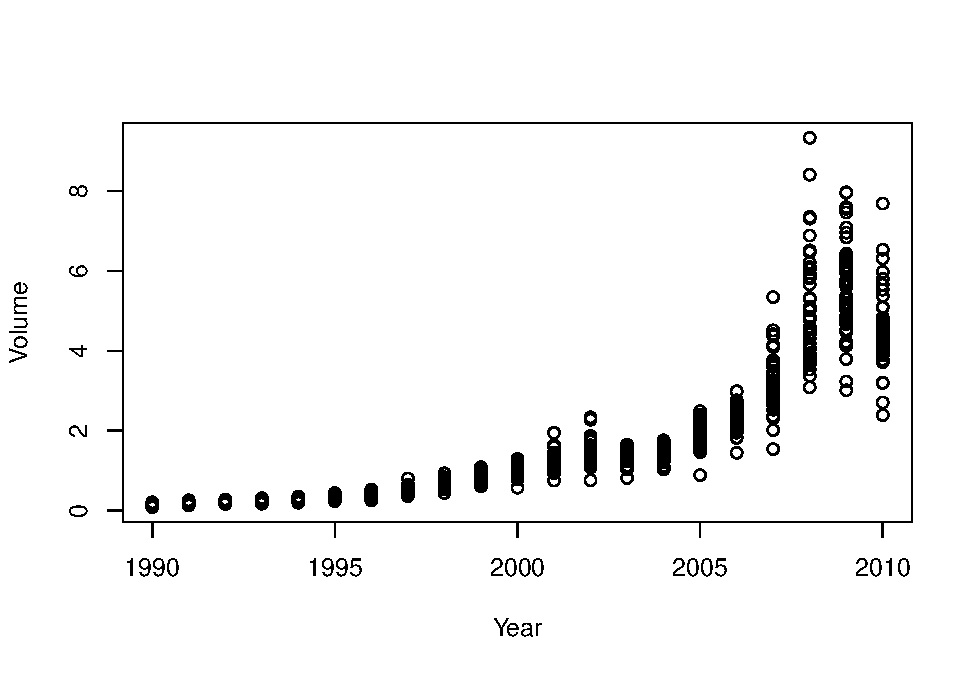
\includegraphics{Homework_09_new_Pan_files/figure-latex/unnamed-chunk-12-1.pdf}
From the correlation matrix, one can find the only the variable
\texttt{Year} and \texttt{Volume} showing the strong correlation. One
possible explanation is that with the development of the global economy,
the number of shares traded also increases.

\begin{Shaded}
\begin{Highlighting}[]
\SpecialCharTok{\textgreater{}} \FunctionTok{pairs}\NormalTok{(Weekly[,}\SpecialCharTok{{-}}\DecValTok{9}\NormalTok{])}
\end{Highlighting}
\end{Shaded}

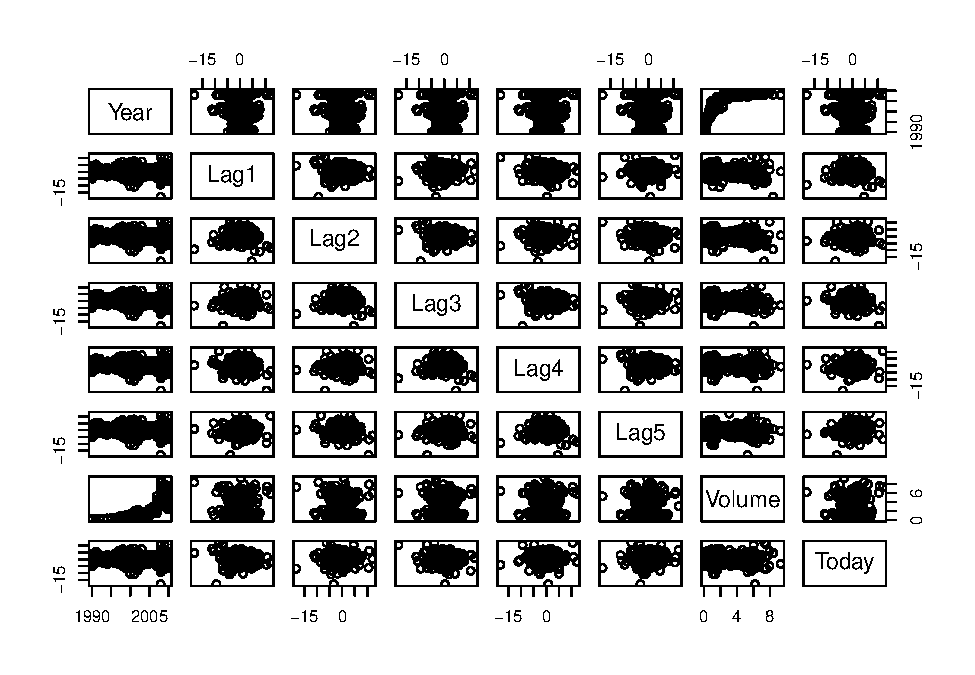
\includegraphics{Homework_09_new_Pan_files/figure-latex/unnamed-chunk-13-1.pdf}
Here, I also checked the scatterplot matrix. It indicates that the
strong correlation might only occurs on \texttt{Year} and
\texttt{Volume}.

\hypertarget{buse-the-full-data-set-to-perform-a-logistic-regression-with-direction-as-the-response-and-the-five-lag-variables-plus-volume-as-predictors.-use-the-summary-function-to-print-the-results.-do-any-of-the-predictors-appear-to-be-statistically-significant-if-so-which-ones}{%
\subsubsection{\texorpdfstring{\textbf{(b)Use the full data set to
perform a logistic regression with Direction as the response and the
five lag variables plus Volume as predictors. Use the summary function
to print the results. Do any of the predictors appear to be
statistically significant? If so, which
ones?}}{(b)Use the full data set to perform a logistic regression with Direction as the response and the five lag variables plus Volume as predictors. Use the summary function to print the results. Do any of the predictors appear to be statistically significant? If so, which ones?}}\label{buse-the-full-data-set-to-perform-a-logistic-regression-with-direction-as-the-response-and-the-five-lag-variables-plus-volume-as-predictors.-use-the-summary-function-to-print-the-results.-do-any-of-the-predictors-appear-to-be-statistically-significant-if-so-which-ones}}

\textbf{MY SOLUTION}

\begin{Shaded}
\begin{Highlighting}[]
\SpecialCharTok{\textgreater{}} \CommentTok{\# run the logistic model using glm() function}
\ErrorTok{\textgreater{}} \FunctionTok{colnames}\NormalTok{(Weekly)}
\NormalTok{[}\DecValTok{1}\NormalTok{] }\StringTok{"Year"}      \StringTok{"Lag1"}      \StringTok{"Lag2"}      \StringTok{"Lag3"}      \StringTok{"Lag4"}      \StringTok{"Lag5"}     
\NormalTok{[}\DecValTok{7}\NormalTok{] }\StringTok{"Volume"}    \StringTok{"Today"}     \StringTok{"Direction"}
\SpecialCharTok{\textgreater{}}\NormalTok{ model\_logi }\OtherTok{\textless{}{-}} \FunctionTok{glm}\NormalTok{(Direction }\SpecialCharTok{\textasciitilde{}}\NormalTok{ Lag1}\SpecialCharTok{+}\NormalTok{Lag2}\SpecialCharTok{+}\NormalTok{Lag3}\SpecialCharTok{+}\NormalTok{Lag4}\SpecialCharTok{+}\NormalTok{Lag5}\SpecialCharTok{+}\NormalTok{Volume,}
\SpecialCharTok{+}                   \AttributeTok{data =}\NormalTok{ Weekly, }\AttributeTok{family =}\NormalTok{ binomial)}
\SpecialCharTok{\textgreater{}} \FunctionTok{summary}\NormalTok{(model\_logi)}

\NormalTok{Call}\SpecialCharTok{:}
\FunctionTok{glm}\NormalTok{(}\AttributeTok{formula =}\NormalTok{ Direction }\SpecialCharTok{\textasciitilde{}}\NormalTok{ Lag1 }\SpecialCharTok{+}\NormalTok{ Lag2 }\SpecialCharTok{+}\NormalTok{ Lag3 }\SpecialCharTok{+}\NormalTok{ Lag4 }\SpecialCharTok{+}\NormalTok{ Lag5 }\SpecialCharTok{+} 
\NormalTok{    Volume, }\AttributeTok{family =}\NormalTok{ binomial, }\AttributeTok{data =}\NormalTok{ Weekly)}

\NormalTok{Deviance Residuals}\SpecialCharTok{:} 
\NormalTok{    Min       1Q   Median       3Q      Max  }
\SpecialCharTok{{-}}\FloatTok{1.6949}  \SpecialCharTok{{-}}\FloatTok{1.2565}   \FloatTok{0.9913}   \FloatTok{1.0849}   \FloatTok{1.4579}  

\NormalTok{Coefficients}\SpecialCharTok{:}
\NormalTok{            Estimate Std. Error z value }\FunctionTok{Pr}\NormalTok{(}\SpecialCharTok{\textgreater{}}\ErrorTok{|}\NormalTok{z}\SpecialCharTok{|}\NormalTok{)   }
\NormalTok{(Intercept)  }\FloatTok{0.26686}    \FloatTok{0.08593}   \FloatTok{3.106}   \FloatTok{0.0019} \SpecialCharTok{**}
\NormalTok{Lag1        }\SpecialCharTok{{-}}\FloatTok{0.04127}    \FloatTok{0.02641}  \SpecialCharTok{{-}}\FloatTok{1.563}   \FloatTok{0.1181}   
\NormalTok{Lag2         }\FloatTok{0.05844}    \FloatTok{0.02686}   \FloatTok{2.175}   \FloatTok{0.0296} \SpecialCharTok{*} 
\NormalTok{Lag3        }\SpecialCharTok{{-}}\FloatTok{0.01606}    \FloatTok{0.02666}  \SpecialCharTok{{-}}\FloatTok{0.602}   \FloatTok{0.5469}   
\NormalTok{Lag4        }\SpecialCharTok{{-}}\FloatTok{0.02779}    \FloatTok{0.02646}  \SpecialCharTok{{-}}\FloatTok{1.050}   \FloatTok{0.2937}   
\NormalTok{Lag5        }\SpecialCharTok{{-}}\FloatTok{0.01447}    \FloatTok{0.02638}  \SpecialCharTok{{-}}\FloatTok{0.549}   \FloatTok{0.5833}   
\NormalTok{Volume      }\SpecialCharTok{{-}}\FloatTok{0.02274}    \FloatTok{0.03690}  \SpecialCharTok{{-}}\FloatTok{0.616}   \FloatTok{0.5377}   
\SpecialCharTok{{-}{-}{-}}
\NormalTok{Signif. codes}\SpecialCharTok{:}  \DecValTok{0} \StringTok{\textquotesingle{}***\textquotesingle{}} \FloatTok{0.001} \StringTok{\textquotesingle{}**\textquotesingle{}} \FloatTok{0.01} \StringTok{\textquotesingle{}*\textquotesingle{}} \FloatTok{0.05} \StringTok{\textquotesingle{}.\textquotesingle{}} \FloatTok{0.1} \StringTok{\textquotesingle{} \textquotesingle{}} \DecValTok{1}

\NormalTok{(Dispersion parameter }\ControlFlowTok{for}\NormalTok{ binomial family taken to be }\DecValTok{1}\NormalTok{)}

\NormalTok{    Null deviance}\SpecialCharTok{:} \FloatTok{1496.2}\NormalTok{  on }\DecValTok{1088}\NormalTok{  degrees of freedom}
\NormalTok{Residual deviance}\SpecialCharTok{:} \FloatTok{1486.4}\NormalTok{  on }\DecValTok{1082}\NormalTok{  degrees of freedom}
\NormalTok{AIC}\SpecialCharTok{:} \FloatTok{1500.4}

\NormalTok{Number of Fisher Scoring iterations}\SpecialCharTok{:} \DecValTok{4}
\end{Highlighting}
\end{Shaded}

The logistic regression analysis shows that the variable \texttt{Lag2}
is a statistically significant predictor \(p = .030\). That is, one unit
increase in the percentage returns of two days before(i.e.,
\texttt{Lag2}) will be associated with .058 increase in the log-odds of
\texttt{Up} vs.~\texttt{Down}, \(z = 2.175\), \(p=.030\), holding all
other variables constant.

\hypertarget{ccompute-the-confusion-matrix-and-overall-fraction-of-correct-predictions.-explain-what-the-confusion-matrix-is-telling-you-about-the-types-of-mistakes-made-by-logistic-regression.}{%
\subsubsection{\texorpdfstring{\textbf{(c)Compute the confusion matrix
and overall fraction of correct predictions. Explain what the confusion
matrix is telling you about the types of mistakes made by logistic
regression.}}{(c)Compute the confusion matrix and overall fraction of correct predictions. Explain what the confusion matrix is telling you about the types of mistakes made by logistic regression.}}\label{ccompute-the-confusion-matrix-and-overall-fraction-of-correct-predictions.-explain-what-the-confusion-matrix-is-telling-you-about-the-types-of-mistakes-made-by-logistic-regression.}}

\textbf{MY SOLUTION}

First, use the \texttt{predict()} function to get the model-estimated
values of the outcome. Note, the argument \texttt{type\ =\ "response"}
option tells R to output probabilities of the form P(Y = 1\textbar X),
as opposed to other information such as the logit.

\begin{Shaded}
\begin{Highlighting}[]
\SpecialCharTok{\textgreater{}} \CommentTok{\# get the predicted value of the outcome}
\ErrorTok{\textgreater{}}\NormalTok{ model\_logi\_est }\OtherTok{\textless{}{-}} \FunctionTok{predict}\NormalTok{(model\_logi, }\AttributeTok{type =} \StringTok{"response"}\NormalTok{)}
\SpecialCharTok{\textgreater{}} \FunctionTok{round}\NormalTok{(model\_logi\_est[}\DecValTok{1}\SpecialCharTok{:}\DecValTok{20}\NormalTok{],}\DecValTok{3}\NormalTok{)}
    \DecValTok{1}     \DecValTok{2}     \DecValTok{3}     \DecValTok{4}     \DecValTok{5}     \DecValTok{6}     \DecValTok{7}     \DecValTok{8}     \DecValTok{9}    \DecValTok{10}    \DecValTok{11}    \DecValTok{12}    \DecValTok{13} 
\FloatTok{0.609} \FloatTok{0.601} \FloatTok{0.588} \FloatTok{0.482} \FloatTok{0.617} \FloatTok{0.568} \FloatTok{0.579} \FloatTok{0.515} \FloatTok{0.572} \FloatTok{0.555} \FloatTok{0.609} \FloatTok{0.537} \FloatTok{0.513} 
   \DecValTok{14}    \DecValTok{15}    \DecValTok{16}    \DecValTok{17}    \DecValTok{18}    \DecValTok{19}    \DecValTok{20} 
\FloatTok{0.586} \FloatTok{0.625} \FloatTok{0.548} \FloatTok{0.499} \FloatTok{0.593} \FloatTok{0.524} \FloatTok{0.591} 
\end{Highlighting}
\end{Shaded}

The estimated values looks good. Next to change the probabilities into
two direction.

\begin{Shaded}
\begin{Highlighting}[]
\SpecialCharTok{\textgreater{}} \FunctionTok{dim}\NormalTok{(Weekly)}
\NormalTok{[}\DecValTok{1}\NormalTok{] }\DecValTok{1089}    \DecValTok{9}
\SpecialCharTok{\textgreater{}} \CommentTok{\# create a vector of 1089 label "Down"}
\ErrorTok{\textgreater{}}\NormalTok{ pred\_direct }\OtherTok{\textless{}{-}} \FunctionTok{rep}\NormalTok{(}\StringTok{"Down"}\NormalTok{, }\DecValTok{1089}\NormalTok{)}
\SpecialCharTok{\textgreater{}} \CommentTok{\# change the Down to up if the probability is greater than .50}
\ErrorTok{\textgreater{}}\NormalTok{ pred\_direct[model\_logi\_est }\SpecialCharTok{\textgreater{}}\NormalTok{ .}\DecValTok{50}\NormalTok{] }\OtherTok{\textless{}{-}} \StringTok{"Up"}
\SpecialCharTok{\textgreater{}} \CommentTok{\# make a confusion matrix to compare the results}
\ErrorTok{\textgreater{}} \FunctionTok{table}\NormalTok{(pred\_direct, Weekly}\SpecialCharTok{$}\NormalTok{Direction)}
           
\NormalTok{pred\_direct Down  Up}
\NormalTok{       Down   }\DecValTok{54}  \DecValTok{48}
\NormalTok{       Up    }\DecValTok{430} \DecValTok{557}
\SpecialCharTok{\textgreater{}} \CommentTok{\# we can also to get the match rate by }
\ErrorTok{\textgreater{}}\NormalTok{ accuracy }\OtherTok{\textless{}{-}} \FunctionTok{length}\NormalTok{(pred\_direct[}\FunctionTok{which}\NormalTok{(pred\_direct }\SpecialCharTok{==}\NormalTok{ Weekly}\SpecialCharTok{$}\NormalTok{Direction)])}\SpecialCharTok{/} \FunctionTok{nrow}\NormalTok{(Weekly)}
\SpecialCharTok{\textgreater{}}\NormalTok{ accuracy}
\NormalTok{[}\DecValTok{1}\NormalTok{] }\FloatTok{0.5610652}
\end{Highlighting}
\end{Shaded}

In this case, logistic regression correctly predicted the movement of
the market 0.561 of the time.

\hypertarget{dnow-fit-the-logistic-regression-model-using-a-training-data-period-from-1990-to-2008-with-lag2-as-the-only-predictor.-compute-the-confusion-matrix-and-the-overall-fraction-of-correct-predictions-for-the-held-out-data-that-is-the-data-from-2009-and-2010.}{%
\subsubsection{\texorpdfstring{\textbf{(d)Now fit the logistic
regression model using a training data period from 1990 to 2008, with
Lag2 as the only predictor. Compute the confusion matrix and the overall
fraction of correct predictions for the held out data (that is, the data
from 2009 and
2010).}}{(d)Now fit the logistic regression model using a training data period from 1990 to 2008, with Lag2 as the only predictor. Compute the confusion matrix and the overall fraction of correct predictions for the held out data (that is, the data from 2009 and 2010).}}\label{dnow-fit-the-logistic-regression-model-using-a-training-data-period-from-1990-to-2008-with-lag2-as-the-only-predictor.-compute-the-confusion-matrix-and-the-overall-fraction-of-correct-predictions-for-the-held-out-data-that-is-the-data-from-2009-and-2010.}}

\textbf{MY SOLUTION}

\begin{Shaded}
\begin{Highlighting}[]
\SpecialCharTok{\textgreater{}} \FunctionTok{attach}\NormalTok{(Weekly)}
\SpecialCharTok{\textgreater{}} \CommentTok{\# create a vector with T or F values at the length of dataset}
\ErrorTok{\textgreater{}}\NormalTok{ train }\OtherTok{\textless{}{-}}\NormalTok{ (Year }\SpecialCharTok{\textless{}} \DecValTok{2009}\NormalTok{)}
\SpecialCharTok{\textgreater{}} \CommentTok{\# use this vector to subset the train data}
\ErrorTok{\textgreater{}}\NormalTok{ df\_train }\OtherTok{\textless{}{-}}\NormalTok{ Weekly[train,]}
\SpecialCharTok{\textgreater{}}\NormalTok{ df\_test }\OtherTok{\textless{}{-}}\NormalTok{ Weekly[}\SpecialCharTok{!}\NormalTok{train,]}
\SpecialCharTok{\textgreater{}} \CommentTok{\# re{-}run the logistic regression model using only one predictor}
\ErrorTok{\textgreater{}}\NormalTok{ model\_logi2 }\OtherTok{\textless{}{-}} \FunctionTok{glm}\NormalTok{(Direction}\SpecialCharTok{\textasciitilde{}}\NormalTok{ Lag2, }\AttributeTok{data =}\NormalTok{ df\_train, }\AttributeTok{family =}\NormalTok{ binomial)}
\SpecialCharTok{\textgreater{}} \CommentTok{\# get the predicted value on the test dataset.}
\ErrorTok{\textgreater{}}\NormalTok{ model\_logi\_est2 }\OtherTok{\textless{}{-}} \FunctionTok{predict}\NormalTok{(model\_logi2, }\AttributeTok{newdata=}\NormalTok{df\_test, }\AttributeTok{type =} \StringTok{"response"}\NormalTok{)}
\SpecialCharTok{\textgreater{}} \CommentTok{\# change the lable}
\ErrorTok{\textgreater{}}\NormalTok{ pred\_direct2 }\OtherTok{\textless{}{-}} \FunctionTok{ifelse}\NormalTok{(model\_logi\_est2 }\SpecialCharTok{\textgreater{}}\FloatTok{0.5}\NormalTok{, }\StringTok{"Up"}\NormalTok{, }\StringTok{"Down"}\NormalTok{)}
\SpecialCharTok{\textgreater{}} \CommentTok{\# make a confusion matrix to compare the results}
\ErrorTok{\textgreater{}} \FunctionTok{table}\NormalTok{(pred\_direct2, df\_test}\SpecialCharTok{$}\NormalTok{Direction)}
            
\NormalTok{pred\_direct2 Down Up}
\NormalTok{        Down    }\DecValTok{9}  \DecValTok{5}
\NormalTok{        Up     }\DecValTok{34} \DecValTok{56}
\SpecialCharTok{\textgreater{}} \CommentTok{\# we can also to get the match rate by }
\ErrorTok{\textgreater{}}\NormalTok{ accuracy }\OtherTok{\textless{}{-}} \FunctionTok{length}\NormalTok{(pred\_direct2[}\FunctionTok{which}\NormalTok{(pred\_direct2 }\SpecialCharTok{==}\NormalTok{ df\_test}\SpecialCharTok{$}\NormalTok{Direction)])}\SpecialCharTok{/} \FunctionTok{nrow}\NormalTok{(df\_test)}
\SpecialCharTok{\textgreater{}}\NormalTok{ accuracy}
\NormalTok{[}\DecValTok{1}\NormalTok{] }\FloatTok{0.625}
\end{Highlighting}
\end{Shaded}

In this case, logistic regression correctly predicted the movement of
the market 0.625 of the time.

\hypertarget{erepeat-d-using-lda}{%
\subsubsection{\texorpdfstring{\textbf{(e)Repeat (d) using
LDA}}{(e)Repeat (d) using LDA}}\label{erepeat-d-using-lda}}

\textbf{MY SOLUTION}\\
Note LDA/QDA/Naive Bayes all belong to Bayesian Classifier Method with
different distribution assumptions.

The LDA classifier results from assuming that the observation within
each class come from a normal distribution with a class-specific mean
and a common variance, and plugging estimates for these parameters into
the Bayesian classifier.

\begin{Shaded}
\begin{Highlighting}[]
\SpecialCharTok{\textgreater{}} \FunctionTok{library}\NormalTok{(MASS)}
\SpecialCharTok{\textgreater{}} \CommentTok{\# run the LDA model}
\ErrorTok{\textgreater{}}\NormalTok{ lda\_fit }\OtherTok{\textless{}{-}} \FunctionTok{lda}\NormalTok{(Direction}\SpecialCharTok{\textasciitilde{}}\NormalTok{ Lag2, }\AttributeTok{data=}\NormalTok{ df\_train)}
\SpecialCharTok{\textgreater{}} \CommentTok{\# using the esitimated result to run on the test dataset}
\ErrorTok{\textgreater{}} \CommentTok{\# get the predicted value on the test dataset.}
\ErrorTok{\textgreater{}}\NormalTok{ lda\_pred}\OtherTok{\textless{}{-}} \FunctionTok{predict}\NormalTok{(lda\_fit, }\AttributeTok{newdata=}\NormalTok{df\_test)}
\SpecialCharTok{\textgreater{}} \CommentTok{\# change the lable}
\ErrorTok{\textgreater{}}\NormalTok{ lda\_class }\OtherTok{\textless{}{-}}\NormalTok{ lda\_pred}\SpecialCharTok{$}\NormalTok{class}
\SpecialCharTok{\textgreater{}} \FunctionTok{table}\NormalTok{(lda\_class, df\_test}\SpecialCharTok{$}\NormalTok{Direction)}
         
\NormalTok{lda\_class Down Up}
\NormalTok{     Down    }\DecValTok{9}  \DecValTok{5}
\NormalTok{     Up     }\DecValTok{34} \DecValTok{56}
\SpecialCharTok{\textgreater{}} \FunctionTok{mean}\NormalTok{(lda\_class }\SpecialCharTok{==}\NormalTok{ df\_test}\SpecialCharTok{$}\NormalTok{Direction)}
\NormalTok{[}\DecValTok{1}\NormalTok{] }\FloatTok{0.625}
\end{Highlighting}
\end{Shaded}

In this case, LDA correctly predicted the movement of the market 0.625
of the time.

\hypertarget{frepeat-d-using-qda}{%
\subsubsection{\texorpdfstring{\textbf{(f)Repeat (d) using
QDA}}{(f)Repeat (d) using QDA}}\label{frepeat-d-using-qda}}

\textbf{MY SOLUTION}\\
running QDA is similar to LDA.

\begin{Shaded}
\begin{Highlighting}[]
\SpecialCharTok{\textgreater{}} \CommentTok{\# run the QDA model}
\ErrorTok{\textgreater{}} \FunctionTok{library}\NormalTok{(MASS)}
\SpecialCharTok{\textgreater{}}\NormalTok{ qda\_fit }\OtherTok{\textless{}{-}} \FunctionTok{qda}\NormalTok{(Direction}\SpecialCharTok{\textasciitilde{}}\NormalTok{ Lag2, }\AttributeTok{data=}\NormalTok{ df\_train)}
\SpecialCharTok{\textgreater{}} \CommentTok{\# using the esitimated result to run on the test dataset}
\ErrorTok{\textgreater{}} \CommentTok{\# get the predicted value on the test dataset.}
\ErrorTok{\textgreater{}}\NormalTok{ qda\_pred}\OtherTok{\textless{}{-}} \FunctionTok{predict}\NormalTok{(qda\_fit, }\AttributeTok{newdata=}\NormalTok{df\_test)}
\SpecialCharTok{\textgreater{}} \CommentTok{\# change the lable}
\ErrorTok{\textgreater{}}\NormalTok{ qda\_class }\OtherTok{\textless{}{-}}\NormalTok{ qda\_pred}\SpecialCharTok{$}\NormalTok{class}
\SpecialCharTok{\textgreater{}} \FunctionTok{table}\NormalTok{(qda\_class, df\_test}\SpecialCharTok{$}\NormalTok{Direction)}
         
\NormalTok{qda\_class Down Up}
\NormalTok{     Down    }\DecValTok{0}  \DecValTok{0}
\NormalTok{     Up     }\DecValTok{43} \DecValTok{61}
\SpecialCharTok{\textgreater{}} \FunctionTok{mean}\NormalTok{(qda\_class }\SpecialCharTok{==}\NormalTok{ df\_test}\SpecialCharTok{$}\NormalTok{Direction)}
\NormalTok{[}\DecValTok{1}\NormalTok{] }\FloatTok{0.5865385}
\end{Highlighting}
\end{Shaded}

In this case, QDA correctly predicted the movement of the market 0.587
of the time.

\hypertarget{grepeat-d-using-knn-with-k1}{%
\subsubsection{\texorpdfstring{\textbf{(g)Repeat (d) using KNN with
K=1}}{(g)Repeat (d) using KNN with K=1}}\label{grepeat-d-using-knn-with-k1}}

\textbf{MY SOLUTION}\\
Note, \texttt{knn()} function requires four inputs:\\
- A matrix containing the predictors associated with the training
data;\\
- A matrix containing the predictors associated with the data for which
we wish to make predictions;\\
- A vector containing the class labels for the training observations;\\
- A value for K, the number of nearest neighbors to be used by the
classifier.

\begin{Shaded}
\begin{Highlighting}[]
\SpecialCharTok{\textgreater{}} \FunctionTok{library}\NormalTok{(class)}
\SpecialCharTok{\textgreater{}} \CommentTok{\# extract the required inputs}
\ErrorTok{\textgreater{}}\NormalTok{ train.X }\OtherTok{\textless{}{-}}\NormalTok{ df\_train}\SpecialCharTok{$}\NormalTok{Lag2}
\SpecialCharTok{\textgreater{}}\NormalTok{ test.X }\OtherTok{\textless{}{-}}\NormalTok{ df\_test}\SpecialCharTok{$}\NormalTok{Lag2}
\SpecialCharTok{\textgreater{}}\NormalTok{ train.Direction }\OtherTok{\textless{}{-}}\NormalTok{ df\_train}\SpecialCharTok{$}\NormalTok{Direction}
\SpecialCharTok{\textgreater{}} 
\ErrorTok{\textgreater{}} \CommentTok{\#  run KNN}
\ErrorTok{\textgreater{}}\NormalTok{ knn.pred }\OtherTok{\textless{}{-}} \FunctionTok{knn}\NormalTok{(}\FunctionTok{as.matrix}\NormalTok{(train.X), }\FunctionTok{as.matrix}\NormalTok{(test.X), train.Direction, }\AttributeTok{k =} \DecValTok{1}\NormalTok{)}
\SpecialCharTok{\textgreater{}}\NormalTok{ result }\OtherTok{\textless{}{-}} \FunctionTok{round}\NormalTok{(}\FunctionTok{mean}\NormalTok{(knn.pred }\SpecialCharTok{==}\NormalTok{ df\_test}\SpecialCharTok{$}\NormalTok{Direction),}\DecValTok{3}\NormalTok{)}
\SpecialCharTok{\textgreater{}}\NormalTok{ result}
\NormalTok{[}\DecValTok{1}\NormalTok{] }\FloatTok{0.5}
\end{Highlighting}
\end{Shaded}

In this case, KNN correctly predicted the movement of the market 0.5 of
the time.

\hypertarget{hrepeat-d-using-naive-bayes}{%
\subsubsection{\texorpdfstring{\textbf{(h)Repeat (d) using Naive
Bayes}}{(h)Repeat (d) using Naive Bayes}}\label{hrepeat-d-using-naive-bayes}}

\textbf{MY SOLUTION}\\
Remember instead of assuming that these functions belong to a particular
family of distributions, Naive Bayes make a simple assumption: Within
the kth class, the p predictors are independent.

\begin{Shaded}
\begin{Highlighting}[]
\SpecialCharTok{\textgreater{}} \FunctionTok{library}\NormalTok{(e1071)}
\SpecialCharTok{\textgreater{}}\NormalTok{ nb\_fit }\OtherTok{\textless{}{-}} \FunctionTok{naiveBayes}\NormalTok{(Direction }\SpecialCharTok{\textasciitilde{}}\NormalTok{ Lag2,}\AttributeTok{data=}\NormalTok{df\_train)}
\SpecialCharTok{\textgreater{}}\NormalTok{ nb\_class }\OtherTok{\textless{}{-}} \FunctionTok{predict}\NormalTok{(nb\_fit, }\AttributeTok{newdata=}\NormalTok{df\_test)}
\SpecialCharTok{\textgreater{}} \FunctionTok{table}\NormalTok{(nb\_class, df\_test}\SpecialCharTok{$}\NormalTok{Direction)}
        
\NormalTok{nb\_class Down Up}
\NormalTok{    Down    }\DecValTok{0}  \DecValTok{0}
\NormalTok{    Up     }\DecValTok{43} \DecValTok{61}
\SpecialCharTok{\textgreater{}}\NormalTok{ result }\OtherTok{\textless{}{-}} \FunctionTok{mean}\NormalTok{(nb\_class }\SpecialCharTok{==}\NormalTok{ df\_test}\SpecialCharTok{$}\NormalTok{Direction)}
\SpecialCharTok{\textgreater{}}\NormalTok{ result}
\NormalTok{[}\DecValTok{1}\NormalTok{] }\FloatTok{0.5865385}
\end{Highlighting}
\end{Shaded}

In this case, Naive Bayes Classifier correctly predicted the movement of
the market 0.587 of the time.

\hypertarget{iwhich-of-these-methods-appears-to-provide-the-best-results-on-this-data}{%
\subsubsection{\texorpdfstring{\textbf{(i)Which of these methods appears
to provide the best results on this
data}}{(i)Which of these methods appears to provide the best results on this data}}\label{iwhich-of-these-methods-appears-to-provide-the-best-results-on-this-data}}

\textbf{MY SOLUTION}\\
The results show that the logistic regression and LDA has the best
performance.

\hypertarget{jexperiment-with-different-combinations-of-predictors-including-possible-transformations-and-interactions-for-each-of-the-methods.}{%
\subsubsection{\texorpdfstring{\textbf{(j)Experiment with different
combinations of predictors, including possible transformations and
interactions, for each of the methods.
}}{(j)Experiment with different combinations of predictors, including possible transformations and interactions, for each of the methods. }}\label{jexperiment-with-different-combinations-of-predictors-including-possible-transformations-and-interactions-for-each-of-the-methods.}}

\textbf{MY SOLUTION}\\
I try the KNN with different K first.

\begin{Shaded}
\begin{Highlighting}[]
\SpecialCharTok{\textgreater{}}\NormalTok{ y\_pre }\OtherTok{\textless{}{-}} \FunctionTok{c}\NormalTok{()}
\SpecialCharTok{\textgreater{}}\NormalTok{ range\_ }\OtherTok{\textless{}{-}} \FunctionTok{c}\NormalTok{(}\DecValTok{1}\SpecialCharTok{:}\DecValTok{100}\NormalTok{)}
\SpecialCharTok{\textgreater{}} \ControlFlowTok{for}\NormalTok{ (x }\ControlFlowTok{in}\NormalTok{ range\_)\{}
\SpecialCharTok{+}\NormalTok{   knn.pred }\OtherTok{\textless{}{-}} \FunctionTok{knn}\NormalTok{(}\FunctionTok{as.matrix}\NormalTok{(train.X), }\FunctionTok{as.matrix}\NormalTok{(test.X), train.Direction, }\AttributeTok{k =} \DecValTok{1}\NormalTok{)}
\SpecialCharTok{+}\NormalTok{   result }\OtherTok{\textless{}{-}} \FunctionTok{round}\NormalTok{(}\FunctionTok{mean}\NormalTok{(knn.pred }\SpecialCharTok{==}\NormalTok{ df\_test}\SpecialCharTok{$}\NormalTok{Direction),}\DecValTok{3}\NormalTok{)}
\SpecialCharTok{+}\NormalTok{   y\_pre }\OtherTok{\textless{}{-}} \FunctionTok{c}\NormalTok{(y\_pre, result)}
\SpecialCharTok{+}\NormalTok{ \}}
\SpecialCharTok{\textgreater{}} \FunctionTok{plot}\NormalTok{(range\_, y\_pre,}
\SpecialCharTok{+}      \AttributeTok{type =} \StringTok{"l"}\NormalTok{,}\CommentTok{\# to draw a line rather than a spot}
\SpecialCharTok{+}      \AttributeTok{main =} \StringTok{"The Performance of Different K"}\NormalTok{,}
\SpecialCharTok{+}      \AttributeTok{xlab =} \StringTok{"K values"}\NormalTok{,}
\SpecialCharTok{+}      \AttributeTok{ylab =} \StringTok{"The Accuracy"}\NormalTok{)}
\SpecialCharTok{\textgreater{}} \FunctionTok{grid}\NormalTok{()}
\end{Highlighting}
\end{Shaded}

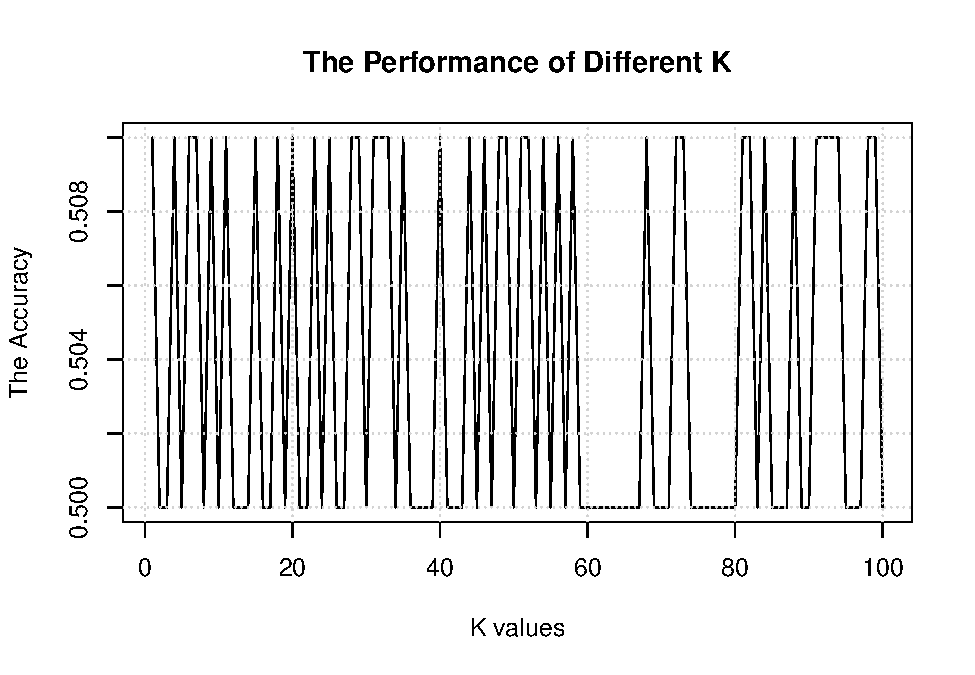
\includegraphics{Homework_09_new_Pan_files/figure-latex/unnamed-chunk-22-1.pdf}
As shown in the plot, with different K, the best accuracy that KNN can
reach is identical. Therefore, I choose K = 1 for parsimony concern.

Next, I will try re-run several model by adding interaction of
\texttt{Lag2} and \texttt{Volume} since the percentage return in the
previous days may affect the investors confidence. Therefore, the
trading volume \texttt{Volume} might depend on that. In addition, I
arbitrarily choose to add the quadratic and cubic form of volume into
the model. I will consider the predictive accuracy as the ultimate
performance criterion.

\begin{Shaded}
\begin{Highlighting}[]
\SpecialCharTok{\textgreater{}} \CommentTok{\# re{-}run the logistic regression analysis}
\ErrorTok{\textgreater{}} \FunctionTok{attach}\NormalTok{(Weekly)}
\SpecialCharTok{\textgreater{}} \CommentTok{\# re{-}run the logistic regression model using only one predictor}
\ErrorTok{\textgreater{}}\NormalTok{ logi\_inter }\OtherTok{\textless{}{-}} \FunctionTok{glm}\NormalTok{(Direction}\SpecialCharTok{\textasciitilde{}}\NormalTok{ Lag2 }\SpecialCharTok{+}\NormalTok{ Volume }\SpecialCharTok{+}\NormalTok{ Lag2}\SpecialCharTok{:}\NormalTok{Volume}\SpecialCharTok{+} \FunctionTok{I}\NormalTok{(Volume}\SpecialCharTok{\^{}}\DecValTok{2}\NormalTok{) }\SpecialCharTok{+} \FunctionTok{I}\NormalTok{(Volume}\SpecialCharTok{\^{}}\DecValTok{3}\NormalTok{), }\AttributeTok{data =}\NormalTok{ df\_train, }\AttributeTok{family =}\NormalTok{ binomial)}
\SpecialCharTok{\textgreater{}} \CommentTok{\# get the summary of the estimation}
\ErrorTok{\textgreater{}} \FunctionTok{summary}\NormalTok{(logi\_inter)}

\NormalTok{Call}\SpecialCharTok{:}
\FunctionTok{glm}\NormalTok{(}\AttributeTok{formula =}\NormalTok{ Direction }\SpecialCharTok{\textasciitilde{}}\NormalTok{ Lag2 }\SpecialCharTok{+}\NormalTok{ Volume }\SpecialCharTok{+}\NormalTok{ Lag2}\SpecialCharTok{:}\NormalTok{Volume }\SpecialCharTok{+} \FunctionTok{I}\NormalTok{(Volume}\SpecialCharTok{\^{}}\DecValTok{2}\NormalTok{) }\SpecialCharTok{+} 
    \FunctionTok{I}\NormalTok{(Volume}\SpecialCharTok{\^{}}\DecValTok{3}\NormalTok{), }\AttributeTok{family =}\NormalTok{ binomial, }\AttributeTok{data =}\NormalTok{ df\_train)}

\NormalTok{Deviance Residuals}\SpecialCharTok{:} 
\NormalTok{   Min      1Q  Median      3Q     Max  }
\SpecialCharTok{{-}}\FloatTok{1.502}  \SpecialCharTok{{-}}\FloatTok{1.260}   \FloatTok{1.020}   \FloatTok{1.088}   \FloatTok{1.538}  

\NormalTok{Coefficients}\SpecialCharTok{:}
\NormalTok{             Estimate Std. Error z value }\FunctionTok{Pr}\NormalTok{(}\SpecialCharTok{\textgreater{}}\ErrorTok{|}\NormalTok{z}\SpecialCharTok{|}\NormalTok{)  }
\NormalTok{(Intercept)  }\FloatTok{0.321744}   \FloatTok{0.139137}   \FloatTok{2.312}   \FloatTok{0.0208} \SpecialCharTok{*}
\NormalTok{Lag2         }\FloatTok{0.048740}   \FloatTok{0.040485}   \FloatTok{1.204}   \FloatTok{0.2286}  
\NormalTok{Volume      }\SpecialCharTok{{-}}\FloatTok{0.163543}   \FloatTok{0.233817}  \SpecialCharTok{{-}}\FloatTok{0.699}   \FloatTok{0.4843}  
\FunctionTok{I}\NormalTok{(Volume}\SpecialCharTok{\^{}}\DecValTok{2}\NormalTok{)  }\FloatTok{0.038516}   \FloatTok{0.088054}   \FloatTok{0.437}   \FloatTok{0.6618}  
\FunctionTok{I}\NormalTok{(Volume}\SpecialCharTok{\^{}}\DecValTok{3}\NormalTok{) }\SpecialCharTok{{-}}\FloatTok{0.003066}   \FloatTok{0.008444}  \SpecialCharTok{{-}}\FloatTok{0.363}   \FloatTok{0.7165}  
\NormalTok{Lag2}\SpecialCharTok{:}\NormalTok{Volume  }\FloatTok{0.002621}   \FloatTok{0.014104}   \FloatTok{0.186}   \FloatTok{0.8526}  
\SpecialCharTok{{-}{-}{-}}
\NormalTok{Signif. codes}\SpecialCharTok{:}  \DecValTok{0} \StringTok{\textquotesingle{}***\textquotesingle{}} \FloatTok{0.001} \StringTok{\textquotesingle{}**\textquotesingle{}} \FloatTok{0.01} \StringTok{\textquotesingle{}*\textquotesingle{}} \FloatTok{0.05} \StringTok{\textquotesingle{}.\textquotesingle{}} \FloatTok{0.1} \StringTok{\textquotesingle{} \textquotesingle{}} \DecValTok{1}

\NormalTok{(Dispersion parameter }\ControlFlowTok{for}\NormalTok{ binomial family taken to be }\DecValTok{1}\NormalTok{)}

\NormalTok{    Null deviance}\SpecialCharTok{:} \FloatTok{1354.7}\NormalTok{  on }\DecValTok{984}\NormalTok{  degrees of freedom}
\NormalTok{Residual deviance}\SpecialCharTok{:} \FloatTok{1349.1}\NormalTok{  on }\DecValTok{979}\NormalTok{  degrees of freedom}
\NormalTok{AIC}\SpecialCharTok{:} \FloatTok{1361.1}

\NormalTok{Number of Fisher Scoring iterations}\SpecialCharTok{:} \DecValTok{4}
\SpecialCharTok{\textgreater{}} \CommentTok{\# get the predicted value on the test dataset.}
\ErrorTok{\textgreater{}}\NormalTok{ logi\_est }\OtherTok{\textless{}{-}} \FunctionTok{predict}\NormalTok{(logi\_inter, }\AttributeTok{newdata=}\NormalTok{df\_test, }\AttributeTok{type =} \StringTok{"response"}\NormalTok{)}
\SpecialCharTok{\textgreater{}} \CommentTok{\# change the lable}
\ErrorTok{\textgreater{}}\NormalTok{ logi\_direct }\OtherTok{\textless{}{-}} \FunctionTok{ifelse}\NormalTok{(logi\_est }\SpecialCharTok{\textgreater{}}\FloatTok{0.5}\NormalTok{, }\StringTok{"Up"}\NormalTok{, }\StringTok{"Down"}\NormalTok{)}
\SpecialCharTok{\textgreater{}} \CommentTok{\# make a confusion matrix to compare the results}
\ErrorTok{\textgreater{}} \FunctionTok{table}\NormalTok{(logi\_direct, df\_test}\SpecialCharTok{$}\NormalTok{Direction)}
           
\NormalTok{logi\_direct Down Up}
\NormalTok{       Down   }\DecValTok{12} \DecValTok{13}
\NormalTok{       Up     }\DecValTok{31} \DecValTok{48}
\SpecialCharTok{\textgreater{}} \CommentTok{\# we can also to get the match rate by }
\ErrorTok{\textgreater{}}\NormalTok{ accuracy }\OtherTok{\textless{}{-}} \FunctionTok{length}\NormalTok{(logi\_direct[}\FunctionTok{which}\NormalTok{(logi\_direct }\SpecialCharTok{==}\NormalTok{ df\_test}\SpecialCharTok{$}\NormalTok{Direction)])}\SpecialCharTok{/} \FunctionTok{nrow}\NormalTok{(df\_test)}
\SpecialCharTok{\textgreater{}}\NormalTok{ accuracy}
\NormalTok{[}\DecValTok{1}\NormalTok{] }\FloatTok{0.5769231}
\end{Highlighting}
\end{Shaded}

In this case, logistic regression correctly predicted the movement of
the market 0.577 of the time.

Next, I re-run the LDA, QDA, and Naive Bayes model.

\begin{Shaded}
\begin{Highlighting}[]
\SpecialCharTok{\textgreater{}} \CommentTok{\# run the LDA model}
\ErrorTok{\textgreater{}} \FunctionTok{library}\NormalTok{(MASS)}
\SpecialCharTok{\textgreater{}}\NormalTok{ lda\_fit }\OtherTok{\textless{}{-}} \FunctionTok{lda}\NormalTok{(Direction}\SpecialCharTok{\textasciitilde{}}\NormalTok{ Lag2 }\SpecialCharTok{+}\NormalTok{ Volume }\SpecialCharTok{+}\NormalTok{ Lag2}\SpecialCharTok{:}\NormalTok{Volume}\SpecialCharTok{+} \FunctionTok{I}\NormalTok{(Volume}\SpecialCharTok{\^{}}\DecValTok{2}\NormalTok{) }\SpecialCharTok{+} \FunctionTok{I}\NormalTok{(Volume}\SpecialCharTok{\^{}}\DecValTok{3}\NormalTok{), }\AttributeTok{data=}\NormalTok{ df\_train)}
\SpecialCharTok{\textgreater{}} \CommentTok{\# using the esitimated result to run on the test dataset}
\ErrorTok{\textgreater{}} \CommentTok{\# get the predicted value on the test dataset.}
\ErrorTok{\textgreater{}}\NormalTok{ lda\_pred}\OtherTok{\textless{}{-}} \FunctionTok{predict}\NormalTok{(lda\_fit, }\AttributeTok{newdata=}\NormalTok{df\_test)}
\SpecialCharTok{\textgreater{}} \CommentTok{\# change the lable}
\ErrorTok{\textgreater{}}\NormalTok{ lda\_class }\OtherTok{\textless{}{-}}\NormalTok{ lda\_pred}\SpecialCharTok{$}\NormalTok{class}
\SpecialCharTok{\textgreater{}} \FunctionTok{table}\NormalTok{(lda\_class, df\_test}\SpecialCharTok{$}\NormalTok{Direction)}
         
\NormalTok{lda\_class Down Up}
\NormalTok{     Down   }\DecValTok{13} \DecValTok{13}
\NormalTok{     Up     }\DecValTok{30} \DecValTok{48}
\SpecialCharTok{\textgreater{}} \FunctionTok{mean}\NormalTok{(lda\_class }\SpecialCharTok{==}\NormalTok{ df\_test}\SpecialCharTok{$}\NormalTok{Direction)}
\NormalTok{[}\DecValTok{1}\NormalTok{] }\FloatTok{0.5865385}
\end{Highlighting}
\end{Shaded}

In this case, LDA correctly predicted the movement of the market 0.587
of the time.

\begin{Shaded}
\begin{Highlighting}[]
\SpecialCharTok{\textgreater{}} \CommentTok{\# run the QDA model}
\ErrorTok{\textgreater{}} \FunctionTok{library}\NormalTok{(MASS)}
\SpecialCharTok{\textgreater{}}\NormalTok{ qda\_fit }\OtherTok{\textless{}{-}} \FunctionTok{qda}\NormalTok{(Direction}\SpecialCharTok{\textasciitilde{}}\NormalTok{ Lag2 }\SpecialCharTok{+}\NormalTok{ Volume }\SpecialCharTok{+}\NormalTok{ Lag2}\SpecialCharTok{:}\NormalTok{Volume}\SpecialCharTok{+} \FunctionTok{I}\NormalTok{(Volume}\SpecialCharTok{\^{}}\DecValTok{2}\NormalTok{) }\SpecialCharTok{+} \FunctionTok{I}\NormalTok{(Volume}\SpecialCharTok{\^{}}\DecValTok{3}\NormalTok{), }\AttributeTok{data=}\NormalTok{ df\_train)}
\SpecialCharTok{\textgreater{}} \CommentTok{\# using the esitimated result to run on the test dataset}
\ErrorTok{\textgreater{}} \CommentTok{\# get the predicted value on the test dataset.}
\ErrorTok{\textgreater{}}\NormalTok{ qda\_pred}\OtherTok{\textless{}{-}} \FunctionTok{predict}\NormalTok{(qda\_fit, }\AttributeTok{newdata=}\NormalTok{df\_test)}
\SpecialCharTok{\textgreater{}} \CommentTok{\# change the lable}
\ErrorTok{\textgreater{}}\NormalTok{ qda\_class }\OtherTok{\textless{}{-}}\NormalTok{ qda\_pred}\SpecialCharTok{$}\NormalTok{class}
\SpecialCharTok{\textgreater{}} \FunctionTok{table}\NormalTok{(qda\_class, df\_test}\SpecialCharTok{$}\NormalTok{Direction)}
         
\NormalTok{qda\_class Down Up}
\NormalTok{     Down   }\DecValTok{31} \DecValTok{45}
\NormalTok{     Up     }\DecValTok{12} \DecValTok{16}
\SpecialCharTok{\textgreater{}} \FunctionTok{mean}\NormalTok{(qda\_class }\SpecialCharTok{==}\NormalTok{ df\_test}\SpecialCharTok{$}\NormalTok{Direction)}
\NormalTok{[}\DecValTok{1}\NormalTok{] }\FloatTok{0.4519231}
\end{Highlighting}
\end{Shaded}

In this case, QDA correctly predicted the movement of the market 0.452
of the time.

Note, the Bayes classier cannot handle the interaction term! I removed
the interaction term in the model.

\begin{Shaded}
\begin{Highlighting}[]
\SpecialCharTok{\textgreater{}} \FunctionTok{library}\NormalTok{(e1071)}
\SpecialCharTok{\textgreater{}}\NormalTok{ nb\_fit }\OtherTok{\textless{}{-}} \FunctionTok{naiveBayes}\NormalTok{(Direction}\SpecialCharTok{\textasciitilde{}}\NormalTok{ Lag2 }\SpecialCharTok{+}\NormalTok{ Volume }\SpecialCharTok{+} \FunctionTok{I}\NormalTok{(Volume}\SpecialCharTok{\^{}}\DecValTok{2}\NormalTok{) }\SpecialCharTok{+} \FunctionTok{I}\NormalTok{(Volume}\SpecialCharTok{\^{}}\DecValTok{3}\NormalTok{),}\AttributeTok{data=}\NormalTok{df\_train)}
\SpecialCharTok{\textgreater{}}\NormalTok{ nb\_class }\OtherTok{\textless{}{-}} \FunctionTok{predict}\NormalTok{(nb\_fit, }\AttributeTok{newdata=}\NormalTok{df\_test)}
\SpecialCharTok{\textgreater{}} \FunctionTok{table}\NormalTok{(nb\_class, df\_test}\SpecialCharTok{$}\NormalTok{Direction)}
        
\NormalTok{nb\_class Down Up}
\NormalTok{    Down   }\DecValTok{43} \DecValTok{57}
\NormalTok{    Up      }\DecValTok{0}  \DecValTok{4}
\SpecialCharTok{\textgreater{}}\NormalTok{ result }\OtherTok{\textless{}{-}} \FunctionTok{mean}\NormalTok{(nb\_class }\SpecialCharTok{==}\NormalTok{ df\_test}\SpecialCharTok{$}\NormalTok{Direction)}
\SpecialCharTok{\textgreater{}}\NormalTok{ result}
\NormalTok{[}\DecValTok{1}\NormalTok{] }\FloatTok{0.4519231}
\end{Highlighting}
\end{Shaded}

In this case, Naive Bayes Classifier correctly predicted the movement of
the market 0.452 of the time.

In conclusion, LDA has the best predictive accuracy 0.587 among these
models. Comparing to the models in previous section, selecting the
appropriate predictors in the right form is critical for model's
performance. One should notice that it might not be a good choice to add
as many as possible predictors to your model.

This dataset is obviously in a time-series form. Maybe some more
advanced and flexible methods can be tested on this dataset, like long
short-term memory networks (LSTM) model, although the model will become
less interpretable. If I finished my class works, I will try run this
analysis on Google Colab via Python.

\end{document}
